%%%%%%%%%%%%%%%%%%%%%%%%%%%%%%%%%%%%%%%%%%%%%%%%%%%%%%%%%%%%%%%%%%%%%
%% This is a (brief) model paper using the achemso class
%% The document class accepts keyval options, which should include
%% the target journal and optionally the manuscript type. 
%%%%%%%%%%%%%%%%%%%%%%%%%%%%%%%%%%%%%%%%%%%%%%%%%%%%%%%%%%%%%%%%%%%%%

%Let's submit to:
%Journal of Medicinal Chemistry will announce a Special Issue on "Artificial Intelligence in Drug Discovery" 

\documentclass[journal=jmcmar,manuscript=article]{achemso}


%%%%%%%%%%%%%%%%%%%%%%%%%%%%%%%%%%%%%%%%%%%%%%%%%%%%%%%%%%%%%%%%%%%%%
%% Place any additional packages needed here.  Only include packages
%% which are essential, to avoid problems later. Do NOT use any
%% packages which require e-TeX (for example etoolbox): the e-TeX
%% extensions are not currently available on the ACS conversion
%% servers.
%%%%%%%%%%%%%%%%%%%%%%%%%%%%%%%%%%%%%%%%%%%%%%%%%%%%%%%%%%%%%%%%%%%%%
\usepackage[version=3]{mhchem} % Formula subscripts using \ce{}
\usepackage{subcaption}
\usepackage{array}
\usepackage{url}
\usepackage{xr-hyper}
\usepackage{hyperref}
\usepackage{multirow}
\usepackage{soul}
\usepackage[flushleft]{threeparttable}
\captionsetup[figure]{font=small,labelfont=small}

\makeatletter
\newcommand*{\addFileDependency}[1]{% argument=file name and extension
  \typeout{(#1)}
  \@addtofilelist{#1}
  \IfFileExists{#1}{}{\typeout{No file #1.}}
}
\setlength\acs@tocentry@height{8.25cm}
\setlength\acs@tocentry@width{4.45cm}
\makeatother
\newcommand*{\myexternaldocument}[1]{%
    \externaldocument{#1}%
    \addFileDependency{#1.tex}%
    \addFileDependency{#1.aux}%
}

\myexternaldocument{supp}

%%%%%%%%%%%%%%%%%%%%%%%%%%%%%%%%%%%%%%%%%%%%%%%%%%%%%%%%%%%%%%%%%%%%%
%% If issues arise when submitting your manuscript, you may want to
%% un-comment the next line.  This provides information on the
%% version of every file you have used.
%%%%%%%%%%%%%%%%%%%%%%%%%%%%%%%%%%%%%%%%%%%%%%%%%%%%%%%%%%%%%%%%%%%%%
%%\listfiles

%%%%%%%%%%%%%%%%%%%%%%%%%%%%%%%%%%%%%%%%%%%%%%%%%%%%%%%%%%%%%%%%%%%%%
%% Place any additional macros here.  Please use \newcommand* where
%% possible, and avoid layout-changing macros (which are not used
%% when typesetting).
%%%%%%%%%%%%%%%%%%%%%%%%%%%%%%%%%%%%%%%%%%%%%%%%%%%%%%%%%%%%%%%%%%%%%
\newcommand*\mycommand[1]{\texttt{\emph{#1}}}


%%%%%%%%%%%%%%%%%%%%%%%%%%%%%%%%%%%%%%%%%%%%%%%%%%%%%%%%%%%%%%%%%%%%%
%% Meta-data block
%% ---------------
%% Each author should be given as a separate \author command.
%%
%% Corresponding authors should have an e-mail given after the author
%% name as an \email command. Phone and fax numbers can be given
%% using \phone and \fax, respectively; this information is optional.
%%
%% The affiliation of authors is given after the authors; each
%% \affiliation command applies to all preceding authors not already
%% assigned an affiliation.
%%
%% The affiliation takes an option argument for the short name.  This
%% will typically be something like "University of Somewhere".
%%
%% The \altaffiliation macro should be used for new address, etc.
%% On the other hand, \alsoaffiliation is used on a per author basis
%% when authors are associated with multiple institutions.
%%%%%%%%%%%%%%%%%%%%%%%%%%%%%%%%%%%%%%%%%%%%%%%%%%%%%%%%%%%%%%%%%%%%%
\author{Paul G. Francoeur}
\author{David R. Koes}
\email{dkoes@pitt.edu}
\affiliation[Pitt]{Department of Computational and Systems Biology, University of Pittsburgh, Pittsburgh, PA 15260}


%%%%%%%%%%%%%%%%%%%%%%%%%%%%%%%%%%%%%%%%%%%%%%%%%%%%%%%%%%%%%%%%%%%%%
%% The document title should be given as usual. Some journals require
%% a running title from the author: this should be supplied as an
%% optional argument to \title.
%%%%%%%%%%%%%%%%%%%%%%%%%%%%%%%%%%%%%%%%%%%%%%%%%%%%%%%%%%%%%%%%%%%%%
\title[TODO]{Need a working title yo}

%%%%%%%%%%%%%%%%%%%%%%%%%%%%%%%%%%%%%%%%%%%%%%%%%%%%%%%%%%%%%%%%%%%%%
%% Some journals require a list of abbreviations or keywords to be
%% supplied. These should be set up here, and will be printed after
%% the title and author information, if needed.
%%%%%%%%%%%%%%%%%%%%%%%%%%%%%%%%%%%%%%%%%%%%%%%%%%%%%%%%%%%%%%%%%%%%%
\keywords{active learning, regression, pKa, molecular property prediction, deep learning, machine learning}

%%%%%%%%%%%%%%%%%%%%%%%%%%%%%%%%%%%%%%%%%%%%%%%%%%%%%%%%%%%%%%%%%%%%%
%% The manuscript does not need to include \maketitle, which is
%% executed automatically.
%%%%%%%%%%%%%%%%%%%%%%%%%%%%%%%%%%%%%%%%%%%%%%%%%%%%%%%%%%%%%%%%%%%%%
\begin{document}

%%%%%%%%%%%%%%%%%%%%%%%%%%%%%%%%%%%%%%%%%%%%%%%%%%%%%%%%%%%%%%%%%%%%%
%% The "tocentry" environment can be used to create an entry for the
%% graphical table of contents. It is given here as some journals
%% require that it is printed as part of the abstract page. It will
%% be automatically moved as appropriate.
%%%%%%%%%%%%%%%%%%%%%%%%%%%%%%%%%%%%%%%%%%%%%%%%%%%%%%%%%%%%%%%%%%%%%
%\begin{tocentry}

% Some journals require a graphical entry for the Table of Contents.
% This should be laid out ``print ready'' so that the sizing of the
% text is correct.

% Inside the \texttt{tocentry} environment, the font used is Helvetica
% 8\,pt, as required by \emph{Journal of the American Chemical
% Society}.

% The surrounding frame is 9\,cm by 3.5\,cm, which is the maximum
% permitted for  \emph{Journal of the American Chemical Society}
% graphical table of content entries. The box will not resize if the
% content is too big: instead it will overflow the edge of the box.

% This box and the associated title will always be printed on a
% separate page at the end of the document.
%\includegraphics{figures/TOC_CD2020.pdf}
%\end{tocentry}

%%%%%%%%%%%%%%%%%%%%%%%%%%%%%%%%%%%%%%%%%%%%%%%%%%%%%%%%%%%%%%%%%%%%%
%% The abstract environment will automatically gobble the contents
%% if an abstract is not used by the target journal.
%%%%%%%%%%%%%%%%%%%%%%%%%%%%%%%%%%%%%%%%%%%%%%%%%%%%%%%%%%%%%%%%%%%%%
\begin{abstract}
need to write lmao

\end{abstract}

%%%%%%%%%%%%%%%%%%%%%%%%%%%%%%%%%

%%%%%%%%%%%%%%%%%%%%%%%%%%%%%%%%%%%%%%%%%%%%%%%%%%%%%%%%%%%%%%%%%%%%%
%% Introduction and Background
%%%%%%%%%%%%%%%%%%%%%%%%%%%%%%%%%%%%%%%%%%%%%%%%%%%%%%%%%%%%%%%%%%%%%
\section{Introduction}

The number of molecules that obey Lipinski's rule-of-five for oral bioavailablity, otherwise referred to as "drug-like" chemical space has been estimated to be $10^{60}$. \cite{lipinski1997experimental,bohacekChemSpace} Even with the availabilty of high-throughput screening to examine 100,000 compounds per day \cite{htsnumbers}, the number of possible molecules remains far to large to be efficiently labeled. While machine learning methods have been widely adapted at predicting various small molecule properties, this constraint on their available training data limits their effectiveness. As such, it is an open question on how to effectively select which unknown molecules to label in order to boost model performance.

Active learning is the field of machine learning research wherein the learning algorithm can query the labels for a new set of data points in order to perform exactly this task. Active learning can be broken into 3 main categories: 1) uncertainty based methods, 2) committee-based methods, and 3) global methods.\cite{alreview1,alreview2}. Uncertainty based methods utilize a model which can predict its own uncertainty about how to label the data. This allows the selection of new data to label by selecting what the most is least confident. Committee-based methods instead use an ensemble of models to predict the labels of the data and the data where the ensemble disagrees the most is the most informative to label. Lastly, global methods, such as expected model change and expected error reduction, utilize models that have been trained with gradient descent to inform which data should be labeled. Active learning has been successful in language modeling\cite{allanguage}, image classification\cite{allanguage}, molecule classification\cite{alcompoundclass}, and lead optimization\cite{alleadop}. 

However, most of the research with these various active learning approaches focuses on classification tasks. There has been comparatively little research on active learning approaches in regression tasks\cite{alreggreedysample,alnigregress}, possibly due to the difficulty in obtaining an accurate prediction of a model's uncertainty during regression. \citet{alnigregress} recently published a framework for active learning for regression tasks by having their model regress to a normal inverse gamma (NIG) distribution instead of a single number. Notably by regressing to 4 numbers via the NIG distribution instead of two, like regressing to a Gaussian distribution, it is possible to disentangle the aleatoric (data) and epistemic (model) uncertainties. \cite{alnigregress} Notably, this allows the model to suggest batches to be labeled based on only its own uncertainty, which is a state of the art method available in classification tasks.\cite{directepistemicunc}. 

\citet{alnigregress} achieved state of the art performance and showcased the ability of their method to succeed in active learning tasks on the QM9 dataset for molecular property prediction. Thus, we sought to adapt their approach and benchmark it against other active learning techniques for predicting small molecule pKa. We analyzed active learning selection by the variance of the predictions of an ensemble of models, the predicted variance of a single model by regressing to a Gaussian, and the epistemic uncertainty of a single model by regressing to a NIG distribution of feed forward neural networks trained on clustered cross validation (CCV) splits of the OPERA pKa dataset \cite{operapKa}. We show that while a greedy selection ordering shows that there is an optimal selection of molecules to achieve maximal performance on a small subset of held out compounds, none of the active learning approaches achieved better performance than selecting from the withheld molecules at random. Source code for our models, training procedure, and scripts for generating the data in this paper is available at \url{https://github.com/francoep/pKa_activelearning}.

%%%%%%%%%%%%%%%%%%%%%%%%%%%%%%%%%%%%%%%%%%%%%%%%%%%%%%%%%%%%%%%%%%%%%
%% Methods
%%%%%%%%%%%%%%%%%%%%%%%%%%%%%%%%%%%%%%%%%%%%%%%%%%%%%%%%%%%%%%%%%%%%%
\section{Methods}
Here we describe our dataset preparation, active learning selection criteria, and model architectures.

\subsection{Dataset}
We utilized the OPERA pKa dataset\cite{operapKa} as it was the largest easily available and labeled dataset for small molecule pKa. Before model training we first standardized the SMILES\cite{smiles} strings using RDkit\cite{rdkit} and removed any duplicates. Then we normalized the pKa's to 0 mean and unit variance. In order to create CCV folds, we utilized the MACCS keys \cite{maccskeys} representation and created clusters using a Tanimoto similarity threshold of 0.8. These clusters were then randomly split into the various datasets described in Table~\ref{tab:datasets}. For each split, there are 5 different generations each made with a different random seed. Additionally, a PCA visualization of the largest cluster and the secondary cluster we selected for improved coverage in later experiments is shown in Figure~\ref{fig:pcaclusters}.

\begin{table}[]
    \centering
    \begin{tabular}{c|c|c|c|c}
    \hline
        Name & Training Size & Withheld Size & Testing Size & External Size \\
    \hline
        CCV & 50 & 4367 & 1104 & -- \\
        Largest Cluster & 50 & 492 & 50 & 4929 \\
        Largest Cluster Validation* & 50 & 442 & 50 & 50 \\
        Clusters 02 & 50 & 690 & 50 & 4731 \\
    \hline
    \end{tabular}
    \caption{Various data splits used in our experiments. The "Largest Cluster Validation" dataset contains the same Training and Testing sets as "Largest Cluster", but 50 randomly chosen molecules form the Withheld set are selected as the "External set" (called Validation later).}
    \label{tab:datasets}
\end{table}

\begin{figure}[tbph]
    \centering
    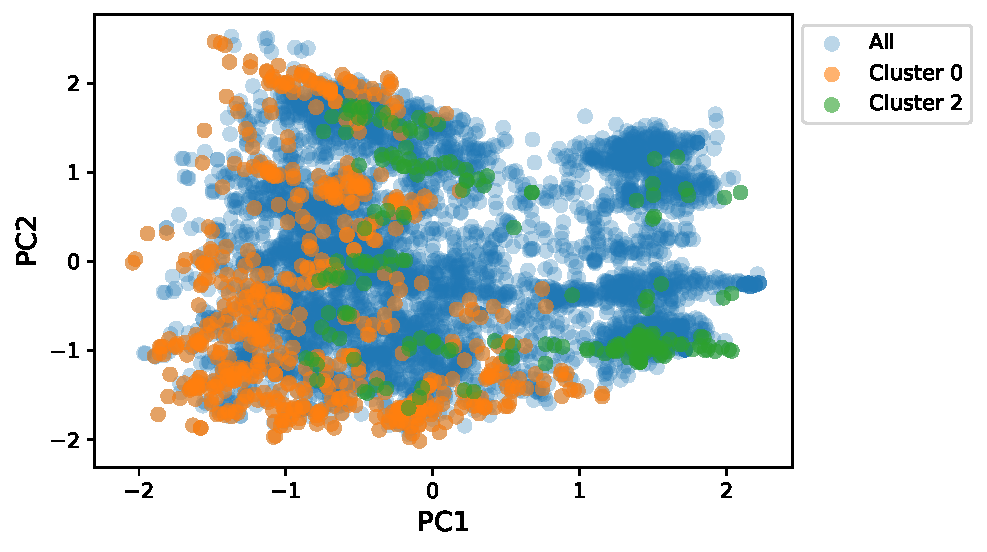
\includegraphics[width=.6\linewidth]{figures/fig1_pca.pdf}
    \caption{Principal Componenets Analysis plot of the Morgan fingerprint with bitsize 2048 of the OPERA pKa dataset. Shownn is the largest and third largest cluster when clustering by MACCS keys using a similarity threshold of 0.8 Tanimoto similarity.}
    \label{fig:pcaclusters}
\end{figure}

\subsection{Active learning selection methods}
The active learning loop is as follows: 1) Train a model from scratch using the available training data and log its performance on the test set, 2) Using the trained model, predict the labels of every molecule in the withheld set, 3) Select the molecule to be added to the training set via a selection criteria, 4) Repeat steps 1-3 until there are no molecules remaining in the withheld set. We investigated 3 strategies for selecting the molecule to add to the training set. In order of increasing complexity we have: 1) Highest variance between the predicted labels of a 5 model ensemble, 2) Highest predicted variance of a single model regressing to a Gaussian distribution, and 3) highest predicted evidence of a single model regressing to a NIG distribution as described by \citet{alnigregress}. We selected these three methods as they represent the naive approach, then a more sophisticated approach, and lastly a state of the art approach to active learning for regression tasks.

For models using the variance of predictions of a 5 model ensemble, each model was trained on the mean-squared error (MSE) of the predicted labels and the true labels of the test set, and only differed between other members of the ensemble by having a different random seed for weight initialization. For the models utilizing the regression to a Gaussian the loss function was log-likelihood of the true label being in the predicted Gaussian distribution. Lastly, for the models regressing to a NIG distribution, we utilized the exact loss defined by \citet{alnigregress}, which is a linear combination of the negative log-likelihood of the true label being in the predicted distribution and the absolute error of the predicted and true labels. Lastly in our later experiments we selected new molecules by the maximal absolute difference of the current predicted label and the previous iteration's predicted label of the molecules in the withheld set.

\subsection{Model architecture}
In order to determine the model architecture we performed a two-stage hyperparameter sweep with weights and biases\cite{wandb} as described in Table~\ref{tab:wandsweep}. Briefly, we selected for the best overall model for each of the two active learning selection methods described above, which turned out to be the same architecture for each loss. Each run of the sweep was performed on the train+validation of a single seed of the CCV data split. Our final architecture is shown in Figure(TODO make). The vast majority of our models were trained on the Morgan fingerprints of the molecule's SMILES with bitsize set to 2048, however we also investigated utilizing a richer input representation to the model. This was done by utilizing the pre-trained molecule attention transformer (MAT) \cite{MAT}, which is a graph transformer that was pre-trained on ChemBL\cite{Chembl} to predict the properties of masked nodes of the input graph. The output of the MAT model is a 1024 dimensional vector, and we fixed the weights to produce this output during our model training.

\begin{figure}[tb]
    \subfloat[Initial Random Sweep]{
        \centering
        \begin{tabular}{|c|c|}
        \hline
            Parameter & Range \\
        \hline
            Fingerprint & RDkit, Morgan, Atompair, Torsions  \\
            Bit Size & 512, 1024, 2048  \\
            Hidden Dimension size & 64,128,256,512  \\
            Loss Functions & MSE, Gaussian log-likelihood, Evidence  \\
            Learning Rate & 0.001, 0.0001, 0.00001  \\
            Number of Hidden Layers & 0,1,2,3  \\
        \hline
        \end{tabular}
        \label{tab:initsweep}
    }
    
    \subfloat[Architecture Refinement]{
        \centering
        \begin{tabular}{|c|c|}
        \hline
            Parameter & Range \\
        \hline
             Fingerprint & RDkit, \textbf{Morgan}\\
             Bit Size & 512, 1024, \textbf{2048}\\
             Epochs & 100, 200, 300, 400 \\
             Hidden Dimension size & 256, 512, \textbf{1024} \\
             Learning Rate & \textbf{0.0001}, 0.00001  \\
             Number of Hidden Layers & 1, \textbf{2}, 3, 4 \\
         \hline
        \end{tabular}
        \label{tab:archsweep}
    }
    \caption{Two stage hyperparameter sweep to define the final architecture. The initial random sweep was performed via using Weights and Bias's random sweeping tool with the target to minimize the test set RMSE. The architecture refinement sweep was a grid search over the listed parameters after the optimizer hyperparameters were set from the first stage. The second sweep outline was performed for each loss function. Our models utilized the hyperparameters in bold. Each run of the sweep used a single seed of the training+withheld set of the CCV data split.}
    \label{tab:wandsweep}
\end{figure}


%%%%%%%%%%%%%%%%%%%%%%%%%%%%%%%%%%%%%%%%%%%%%%%%%%%%%%%%%%%%%%%%%%%%%
%% Results
%%%%%%%%%%%%%%%%%%%%%%%%%%%%%%%%%%%%%%%%%%%%%%%%%%%%%%%%%%%%%%%%%%%%%
\section{Results}

\subsection{Experiment 1 -- Initial attempt looking at all of the data.}
The first experiment we performed was to run our optimized architecture using 3 different criteria for active learning on the CCV dataset. We utilized the variance of 5 models predictions (Ensemble), the predicted variance of a single model that was regressing to a Gaussian distribution (Gaussian), and the predicted epistemic variance of a singular model regressing to a NIG distribution (NIG). Each of these models is compared to selecting molecules form the withheld set at random. 5 experiments were performed, with each experiment using a different random seed and a different CCV data split. The results are shown in Figure~\ref{fig:initialresults}. Notably, each method is doing no better than selecting molecules at random, as shown by the overlapping error bars.

\begin{figure}[tbph]
    \centering
    \begin{subfigure}[b]{0.48\textwidth}
        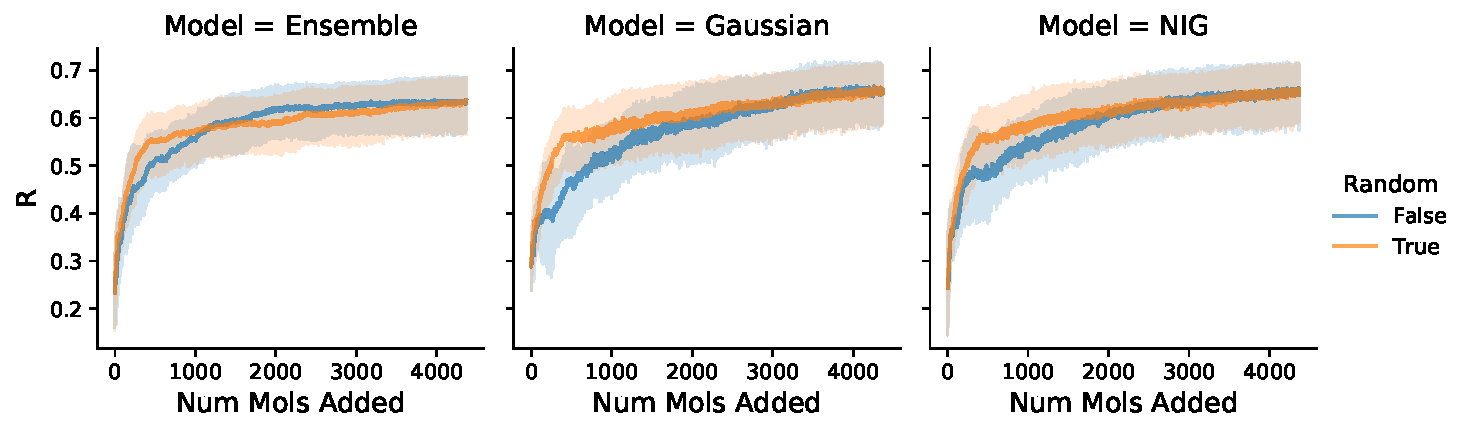
\includegraphics[width=1\linewidth]{figures/fig2_initial_results_R.pdf}
        \caption{Pearson's R correlation on the Test Set}
    \end{subfigure}%
    \hfill
    \begin{subfigure}[b]{0.48\textwidth}
        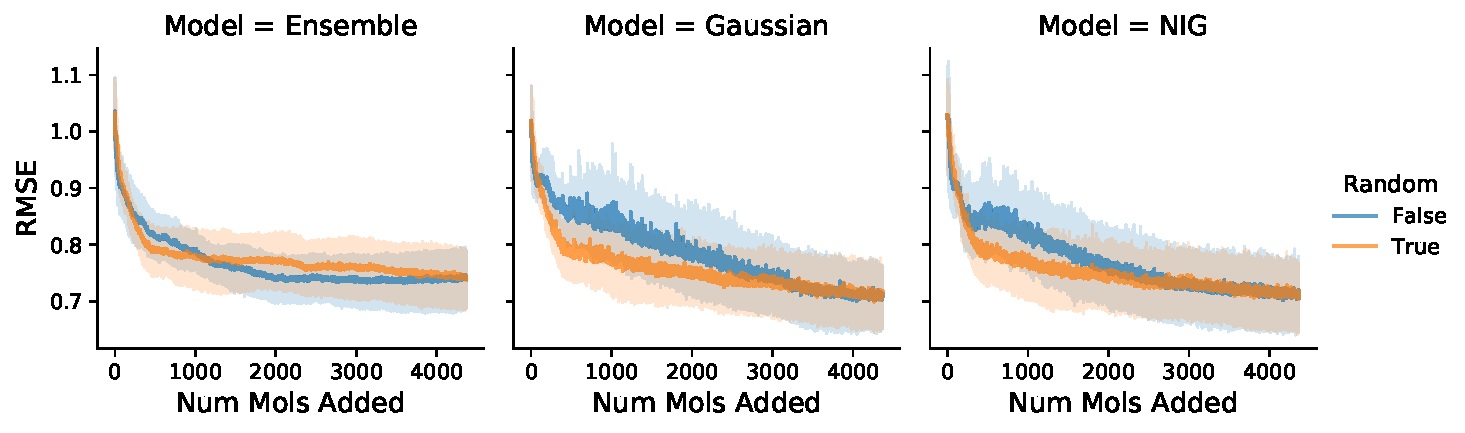
\includegraphics[width=1\linewidth]{figures/fig2_initial_results_RMSE.pdf}
        \caption{RMSE on the Test Set}
    \end{subfigure}
    \caption{Our first experiment testing 3 different active learning methods on the CCV dataset. We ran 5 different seeds, with each seed having it's own split of the CCV data. Ensemble refers to selecting molecules by the maximum variance of the predictions of a 5 model ensemble. Gaussian refers to selecting the maximal predicted variance of a singular model regressing to a Gaussain distribution. Similarly NIG refers to a single model regressing to a NIG distribution and selecting the maximal predicted epistemic variance. Every active learning method is indistinguishable from selecting molecules at random.}
    \label{fig:initialresults}
\end{figure}

\subsection{Experiment 2 -- Restricting to the largest cluster.}
We hypothesized that the failure of the first experiment could be due to the information gain in the CCV dataset being to large. The idea being that since the withheld set contained only molecules that are distinct from the training set due to the clustering, selecing a molecule at random would still provide rich information to a learner as it had never before seen this type of molecule in its prior training. This could allow the random selection to provide a similar information gaining curve in its selection of molecules as the active learning approaches.

In order to test if this is the case, we then repeated the experimental setup but this time only utilized molecules from the largest cluster randomly split into train/withheld/test sets as described in the "Largest Cluster" row of Table~\ref{tab:datasets}. The results of this experiment are shown in Figure~\ref{fig:lcresults}. This experiment also resulted in failure, as every active learning method was indistinguishable from selecting molecules at random to add to the training set.

\begin{figure}[tbph]
    \centering
    \begin{subfigure}[b]{0.48\textwidth}
        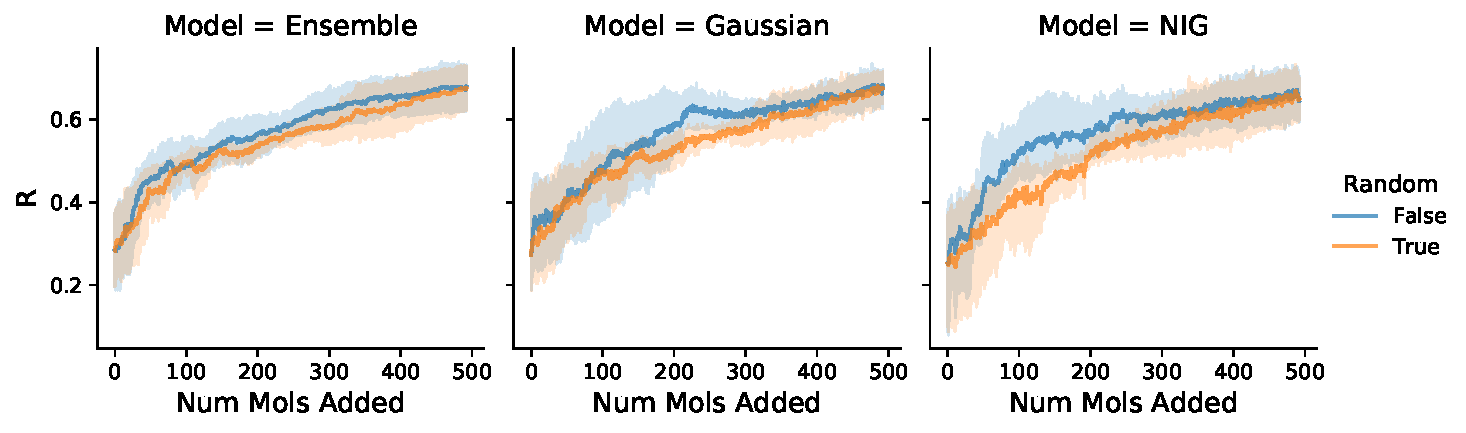
\includegraphics[width=1\linewidth]{figures/fig3_largest_cluster_R.pdf}
        \caption{Pearson's R correlation on the Test Set}
    \end{subfigure}%
    \hfill
    \begin{subfigure}[b]{0.48\textwidth}
        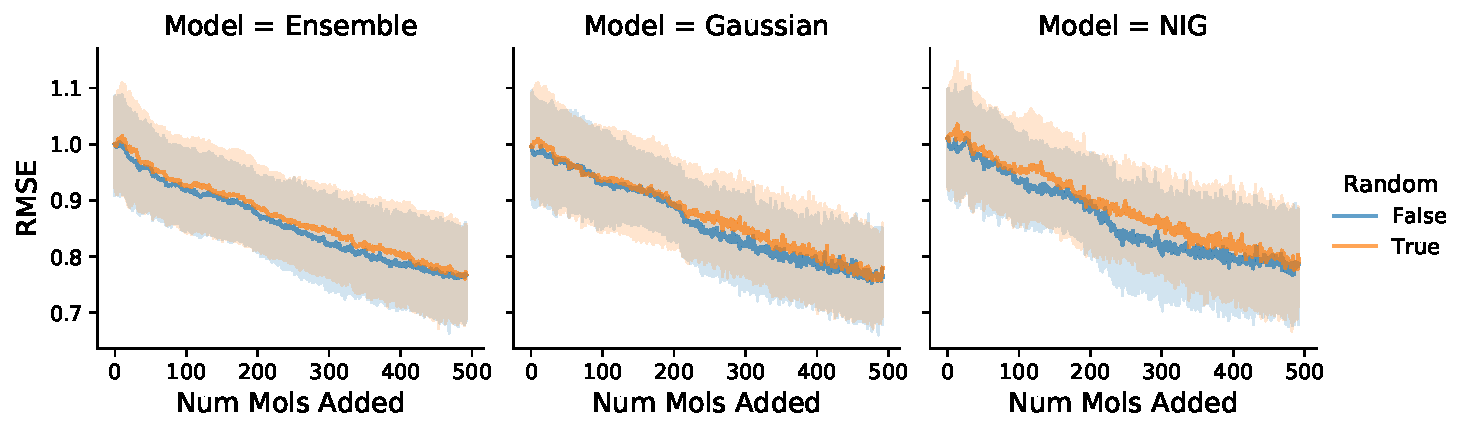
\includegraphics[width=1\linewidth]{figures/fig3_largest_cluster_RMSE.pdf}
        \caption{RMSE on the Test Set}
    \end{subfigure}
    \caption{Our second experiment testing 3 different active learning methods on the Largest Cluster dataset. We ran 5 different seeds, with each seed having it's own random split of the data. The same models that were utilized in Figure~\ref{fig:initialresults} are used here. Again, every active learning method is indistinguishable from selecting molecules at random.}
    \label{fig:lcresults}
\end{figure}

\subsection{Experiment 3 -- Verifying if signal is present in this dataset.}
The failure of the active learning methods to perform better than random molecule selection when we restricted all the data to one cluster suggests that there might not be possible signal present in the data. In order to test this, we need some baseline of maximal performance against which to compare. In order to calculate this baseline we exhaustively train a new model for every molecule in the withheld set during each step of the active learning loop. We then greedily select the molecule to add which resulted in the model that had the lowest RMSE on the test set. This greedy selection by design will have the best possible active learning ordering for whatever test set we are evaluating.

Due to the immense computational burden (having to train $N!$ models where $N$ is the number of molecules in the withheld set), we only performed this analysis on one particular split of the "Largest Cluster" data. The results are shown in Figure~\ref{fig:lcgreed}. We show that for this fold, there does exist an optimal ordering of withheld set molecules that results in a smaller subset of molecules that can acheive the same final performance as adding all of the withheld molecules to the training set. Interestingly, we also show that maximal model performance can be achieved by intentionally not adding all of the withheld molecules, which shows that there are molecules whose addition hurt final model performance. Additionally, models trained only on this cluster of data do not generalize to the out of cluster molecules, as shown by the poor performance on the "Rest" test set, which the models never see during training. Lastly, we point out that while it appears that the active learning methods may be successful in the Pearson's R evaluation on the within cluster test set (orange versus blue lines in Figure\ref{fig:lcgreed}), this effect is an artifact of randomness and disappears with more random seeds as shown in Figure\ref{fig:lcresults}, and that the supposed success is not reflected in the RMSE evaluation.

\begin{figure}[tbph]
    \centering
    \begin{subfigure}[b]{0.48\textwidth}
        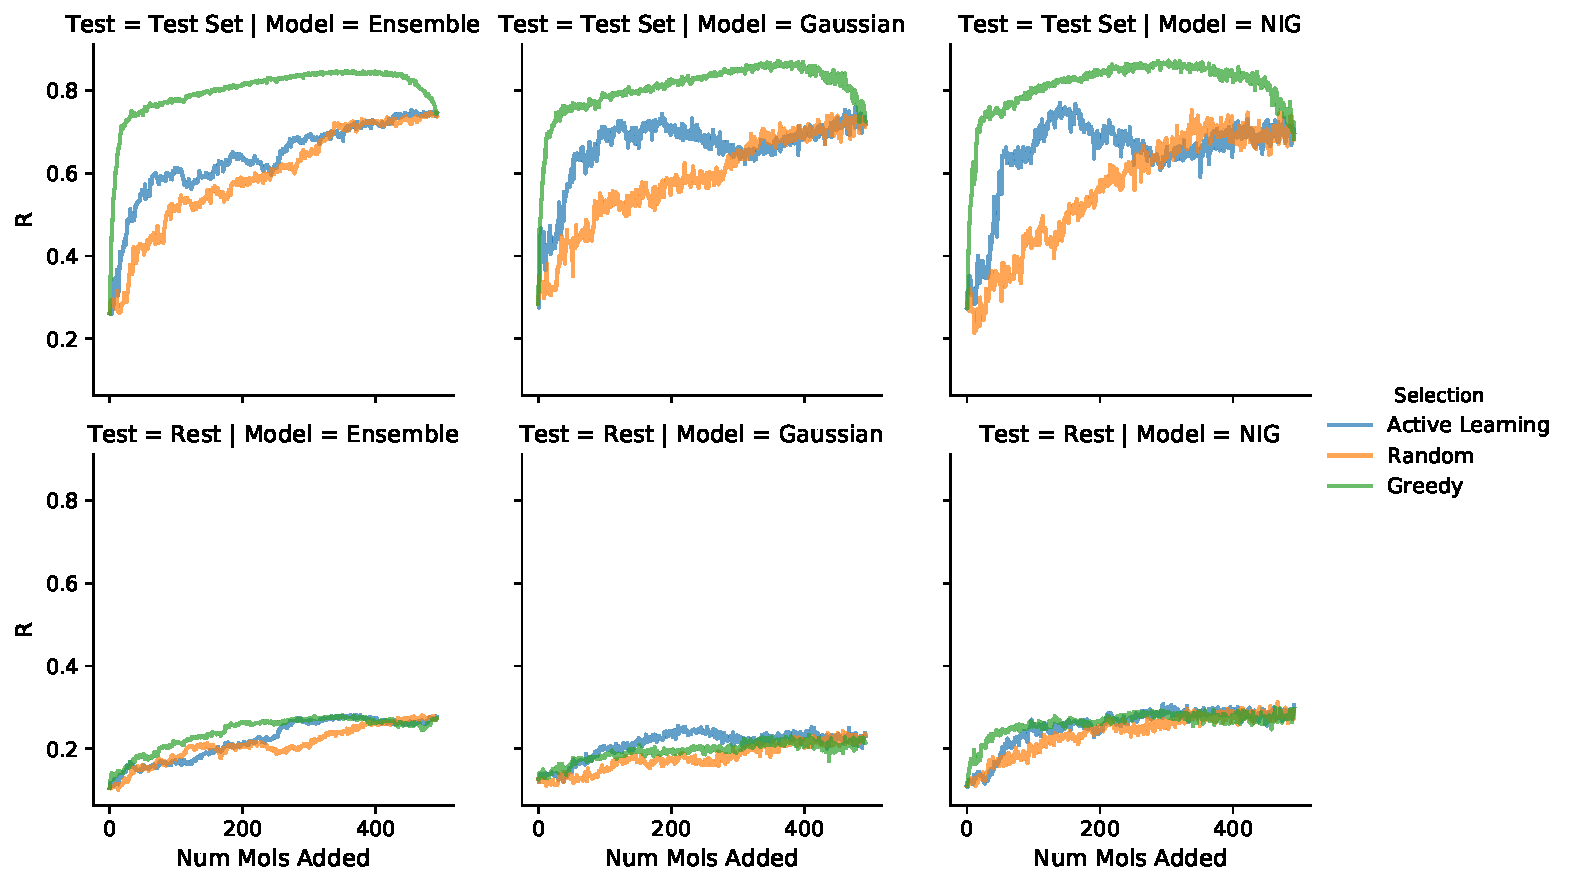
\includegraphics[width=1\linewidth]{figures/fig4_lc_withgreed_R.pdf}
        \caption{Pearson's R correlation on the Test Set}
    \end{subfigure}%
    \hfill
    \begin{subfigure}[b]{0.48\textwidth}
        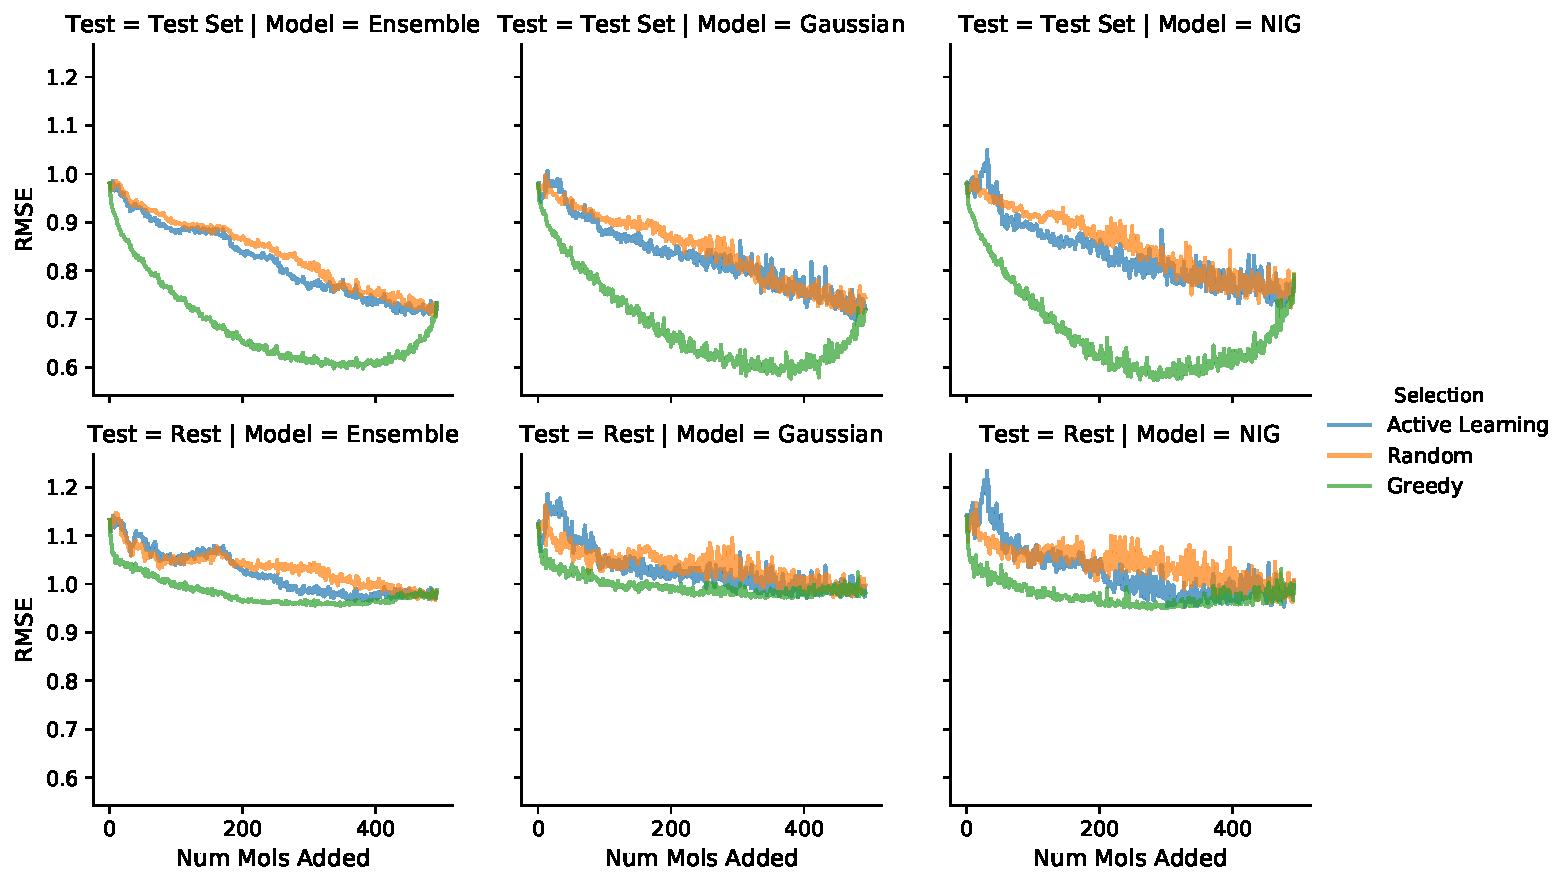
\includegraphics[width=1\linewidth]{figures/fig4_lc_withgreed_RMSE.pdf}
        \caption{RMSE on the Test Set}
    \end{subfigure}
    \caption{Our third experiment testing if an optimal ordering of molecules during an active learning cycle exists on 1 fold of the Largest Cluster dataset. We only ran 1 different seed on 1 fold of the data. The same models that were utilized in Figure~\ref{fig:initialresults} are used here. Notably, there does exist an optimal ordering of molecules for the Test Set. We also report the results of the greedily selected model on the out-of-cluster molecules.}
    \label{fig:lcgreed}
\end{figure}

\subsection{Experiment 4 -- Checking if greedy selection works when selected with a validation set.}

In Experiment 3 we show that performing a Greedy selection with respect to a singular cluster fails to generalize to the other clusters in the dataset. This is unsurprising, as by construction the Greedy selection is overfit to the dataset you are selecting against. Thus, it remains to be shown if fitting to a validation set within a cluster would achieve good results on the test set of said cluster. In order to answer this question we created the "Largest Cluster Validation" set (Table~\ref{tab:datasets}), which consists of the same Training and Testing sets utilized in Experiment 3, but we randomly selected 50 molecules from the Withheld set to serve as our External/Validation set for the Greedy selection algorithm. As in Experiment 3, we trained 1 model with 1 random seed for each of the model types. The results of this experiment are shown in Figure~\ref{fig:lcgreedvalid}. As before we show that an optimal ordering of molecules is identified with the Greedy selection algorithm to provide the fasts final performance on the Validation set. However, this ordering of additional molecules has similar performance to the active learning methods and selecting molecules at random for the Test set. Thus, the Greedy selection algorithm is only useful to provide an upperbound on active learning's performance relative to a particular set of data and does not transfer to other datasets even if they are from the same data cluster.

\begin{figure}[tbph]
    \centering
    \begin{subfigure}[b]{0.48\textwidth}
        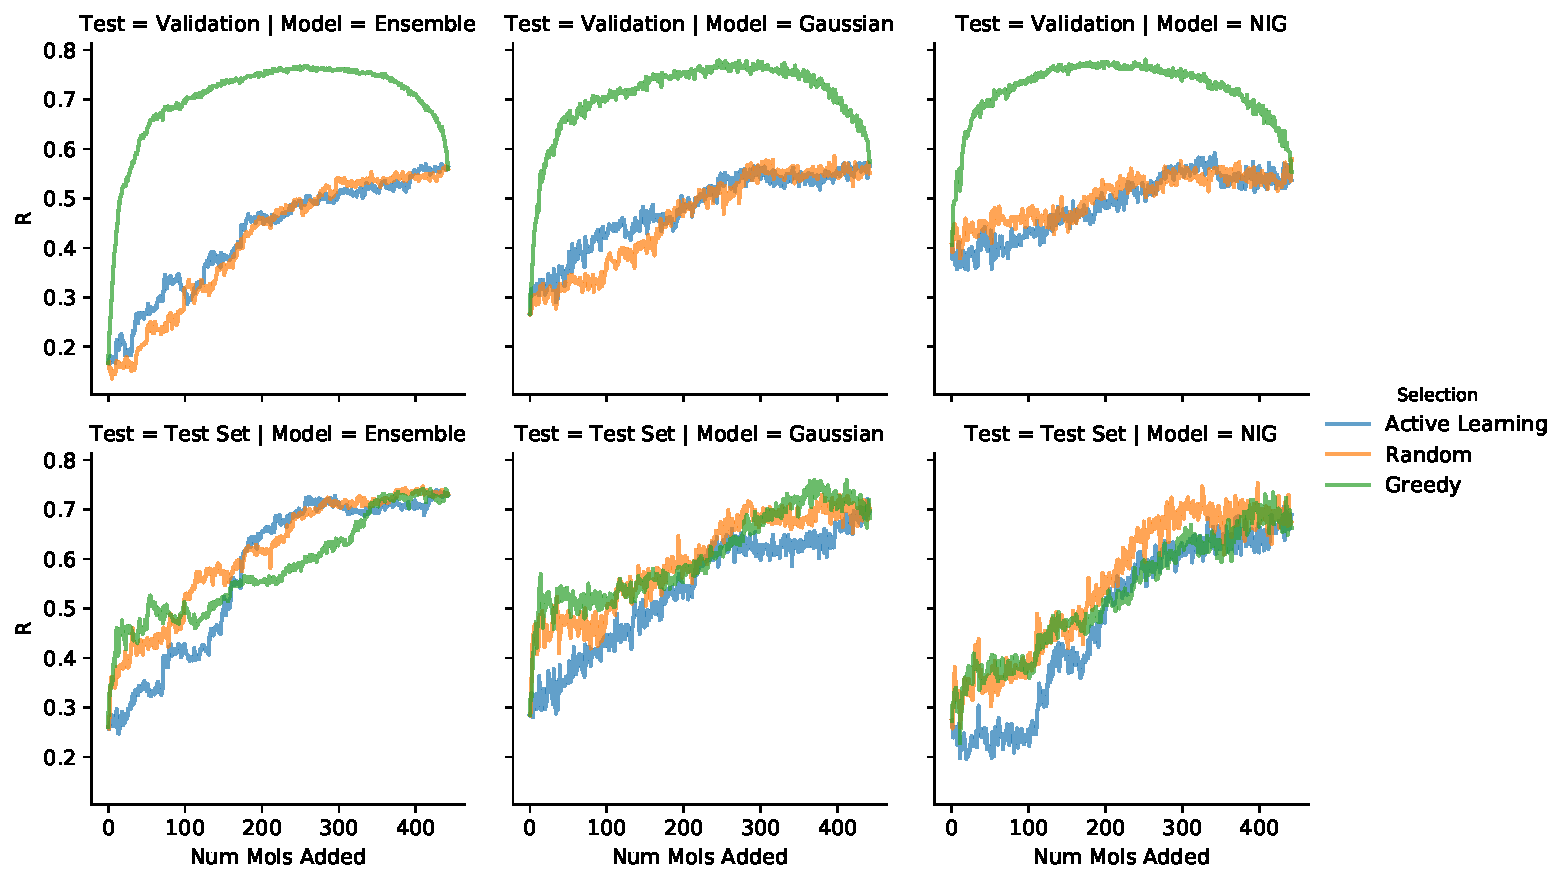
\includegraphics[width=1\linewidth]{figures/fig4a_lc_greed_withvalid_R.pdf}
        \caption{Pearson's R correlation on the Test Set}
    \end{subfigure}%
    \hfill
    \begin{subfigure}[b]{0.48\textwidth}
        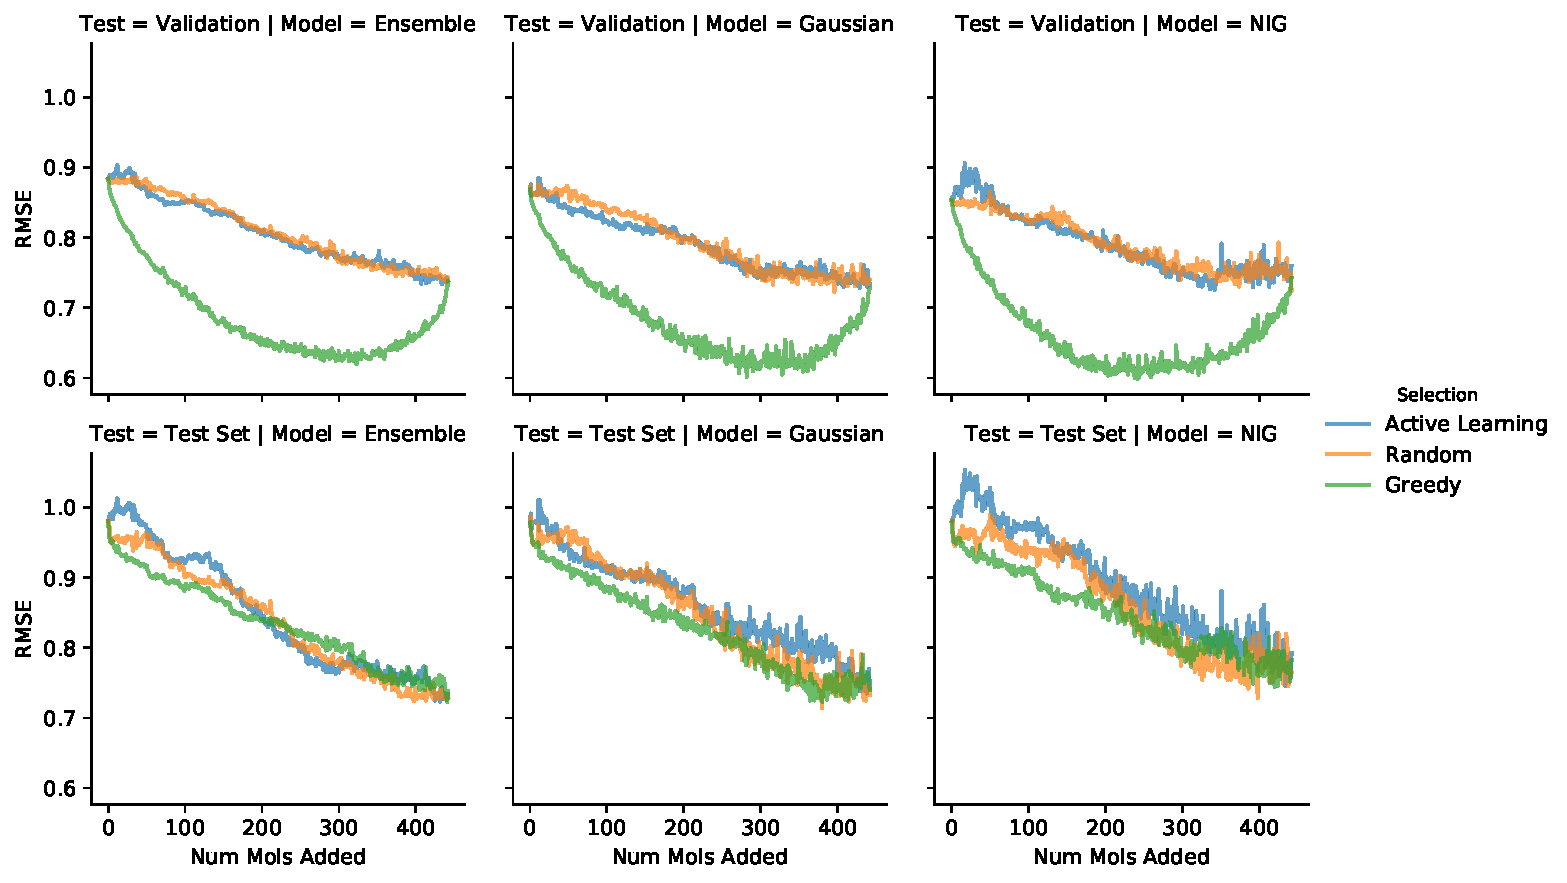
\includegraphics[width=1\linewidth]{figures/fig4a_lc_greed_withvalid_RMSE.pdf}
        \caption{RMSE on the Test Set}
    \end{subfigure}
    \caption{Our fourth experiment checking the results of the greedy ordering when using all within cluster sets. While there exists an optimal ordering of the validation set molecules, the resulting model is no different than random selection on the withheld test set. This experiment was run with 1 seed on 1 fold of the "Largest Cluster Validation" dataset.}
    \label{fig:lcgreedvalid}
\end{figure}

\subsection{Experiment 5 -- Utilizing 2 clusters while regressing to a NIG distribution.}

After showing that an optimal ordering is possible but the active learning approaches still failed in the 1 cluster case, we investigated the 2 cluster case. We selected the third largest cluster as it contained the largest number of molecules while also maximizing the coverage of the chemical space of our model (Figure~\ref{fig:pcaclusters}), and created the "Clusters 02" dataset. The hypothesis is that the addition of the second largest cluster would help the model's ability to generalize and with an extra source of semi-related molecules could have a chance to improve the active learning selection process. We opted to only evaluate the performance of the NIG regression approach and only looked at a single split as we were continuing to use the greedy selection analysis and the larger dataset size constrained our computational resources. The results of this experiment are shown in Figure~\ref{lc02greed}. The addition of the second cluster improved the model's final performance on the test set, and increased the maximal performance of the greedy selection, likely due to having more training data and the same size test set. However, active learning was still no better than randomly picking molecules, and the model saw no improvement on its ability to generalize. Due to both the computational demand, and it not performing well on anything except the dataset it is fit to, we do not perform the Greedy selection baseline on the remainder of our experiments.


\begin{figure}[tbph]
    \centering
    \begin{subfigure}[b]{0.48\textwidth}
        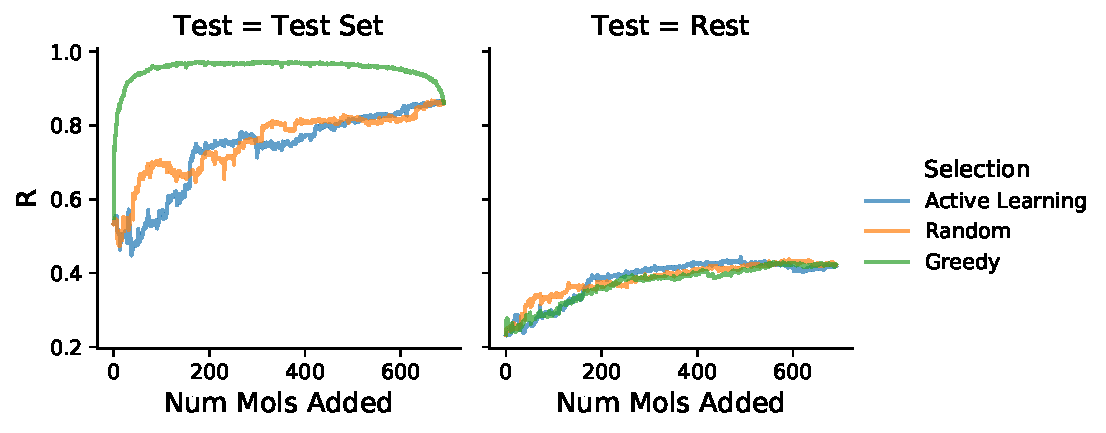
\includegraphics[width=1\linewidth]{figures/fig5_lc02_R.pdf}
        \caption{Pearson's R correlation on the Test Set}
    \end{subfigure}%
    \hfill
    \begin{subfigure}[b]{0.48\textwidth}
        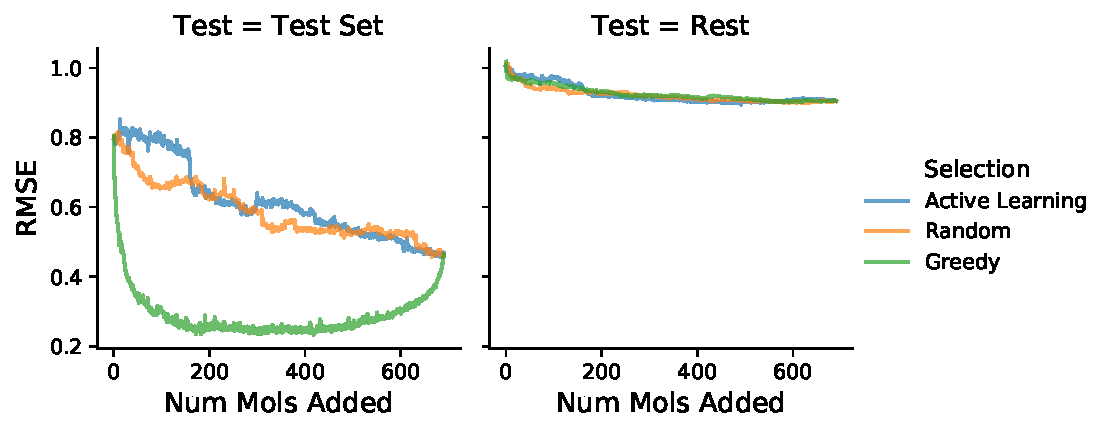
\includegraphics[width=1\linewidth]{figures/fig5_lc02_RMSE.pdf}
        \caption{RMSE on the Test Set}
    \end{subfigure}
    \caption{Our fifth experiment testing the effect of utilizing the Clusters 02 dataset. In this experiment we only ran 1 seed on 1 fold of the data, and only used the NIG regression approach to active learning. In each subplot the within cluster Test set is shown on the left and the performance on all remaining clusters is shown on the right. Again we show that an optimal ordering of the withheld molecules exists for this test set, and that the addition of a second cluster of data did not improve the model's ability to generalize.}
    \label{fig:lc02greed}
\end{figure}

\subsection{Experiment 6 -- Varying the input representations and training times.}

As everything we have tried thus far has failed, we hypothesized that utilizing the Morgan fingerprints as input to our model are not expressive enough for the active learning methods to perform well. Thus we sought to provide a more feature rich input to our model. We selected the pre-trained weights of the MAT\cite{MAT} model as our input representation as the authors were successful in using them on other molecular property prediction tasks, and the pre-training procedure they employed of having the model predict the atom properties of masked nodes would imbue their network with some knowledge of Chemistry. Thus, we hypothesize that by taking the output of the Generator portion of MAT as the input to our model, we could provide a more feature rich input which could boost model performance.

The results of this experiment are shown in Figure~\ref{fig:MATinput}. We also varied our training times by 2 orders of magnitude since our initial sweep which set the model architecture did not utilize this new input in its hyperparameter selection and we do not know how long the model would need to train. We also evaluated every active learning selection criteria with this new input. In general the models trained for only 4 epochs did not learn, the models trained for 40 epochs started to learn, and the models trained for 400 epochs were noisy learners. In terms of RMSE, no active learning method outperformed selecting molecules at random. However, for Pearson's R there is some potential signal in the longer training for the Gaussian and NIG regression models, since there is no difference in the RMSE performance for the same models this is likely misleading. Again, we also observe the failure of these models to generalize outside of the two clusters that they were trained on.

\begin{figure}[tbph]
    \centering
    \begin{subfigure}[b]{0.48\textwidth}
        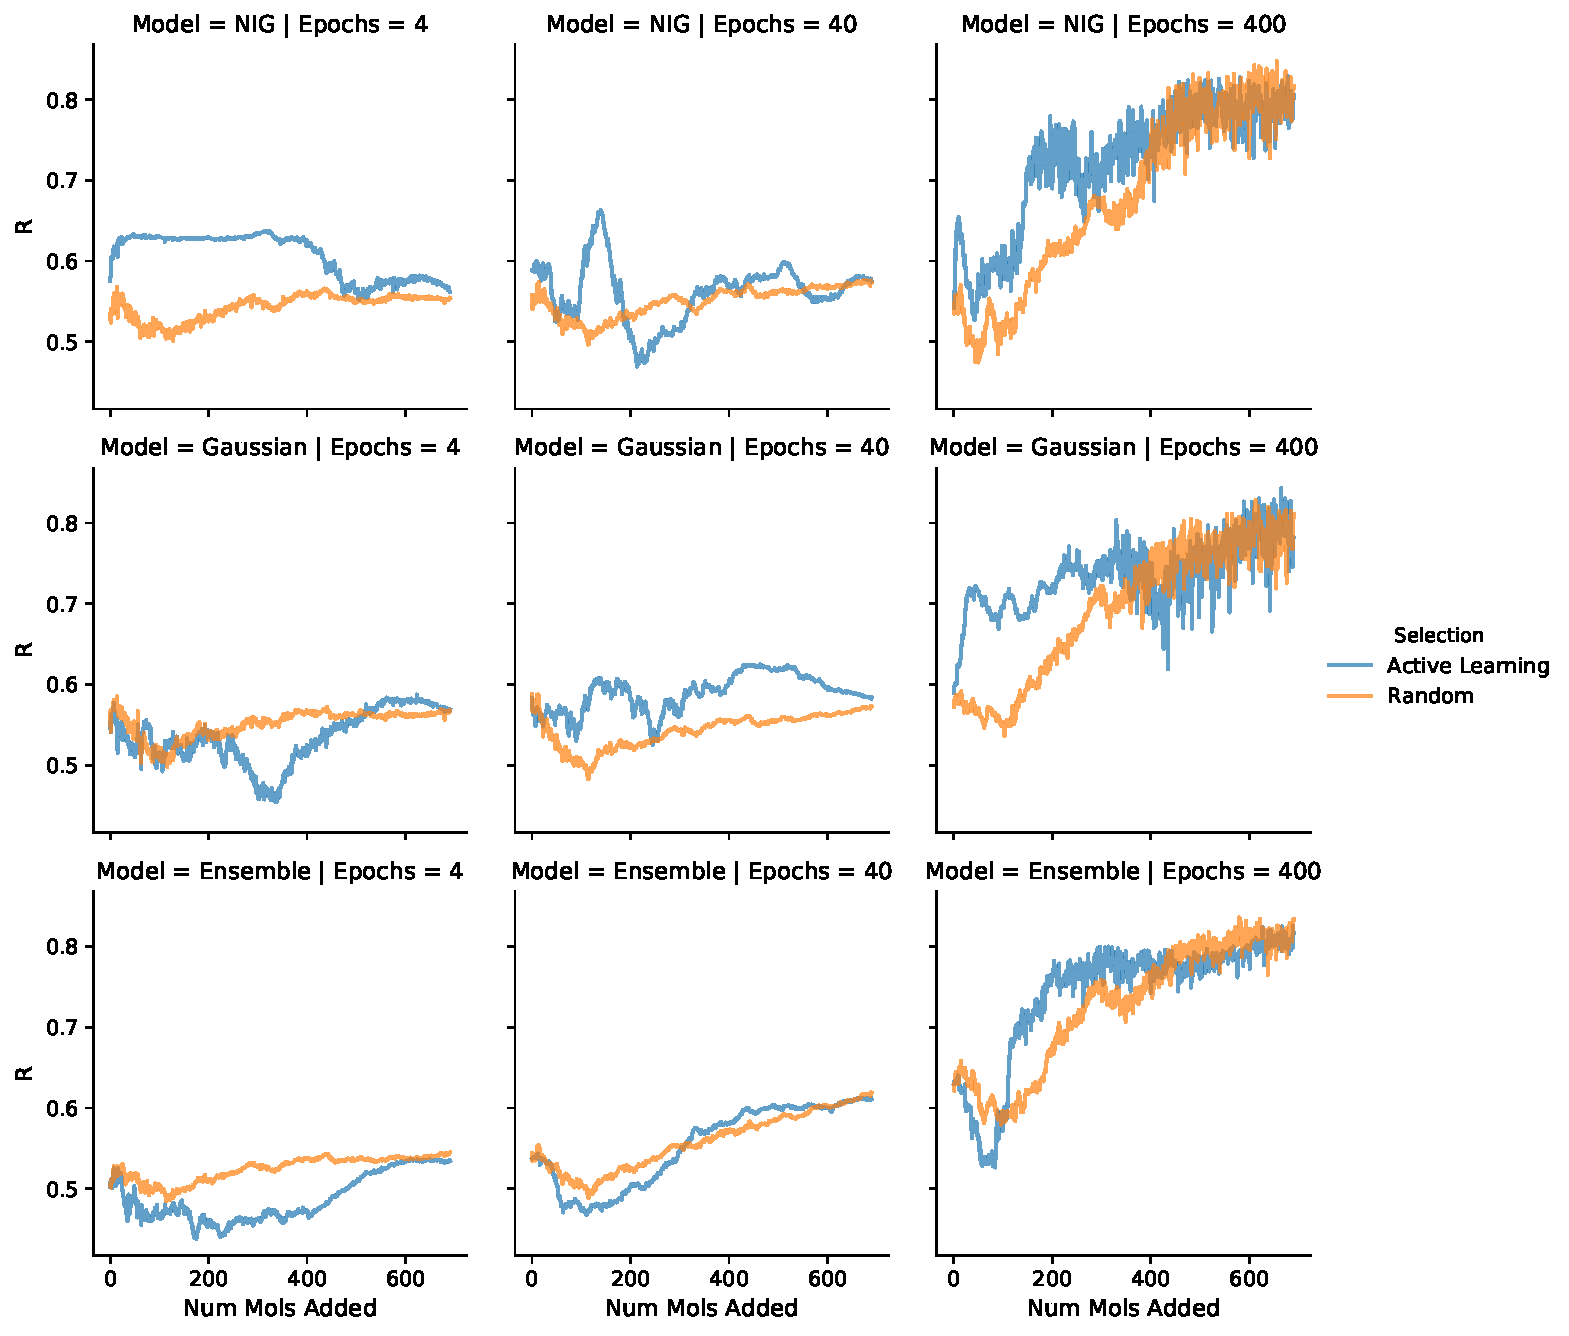
\includegraphics[width=1\linewidth]{figures/fig6_MAT_input_R.pdf}
        \caption{Pearson's R correlation on the Test Set}
    \end{subfigure}%
    \hfill
    \begin{subfigure}[b]{0.48\textwidth}
        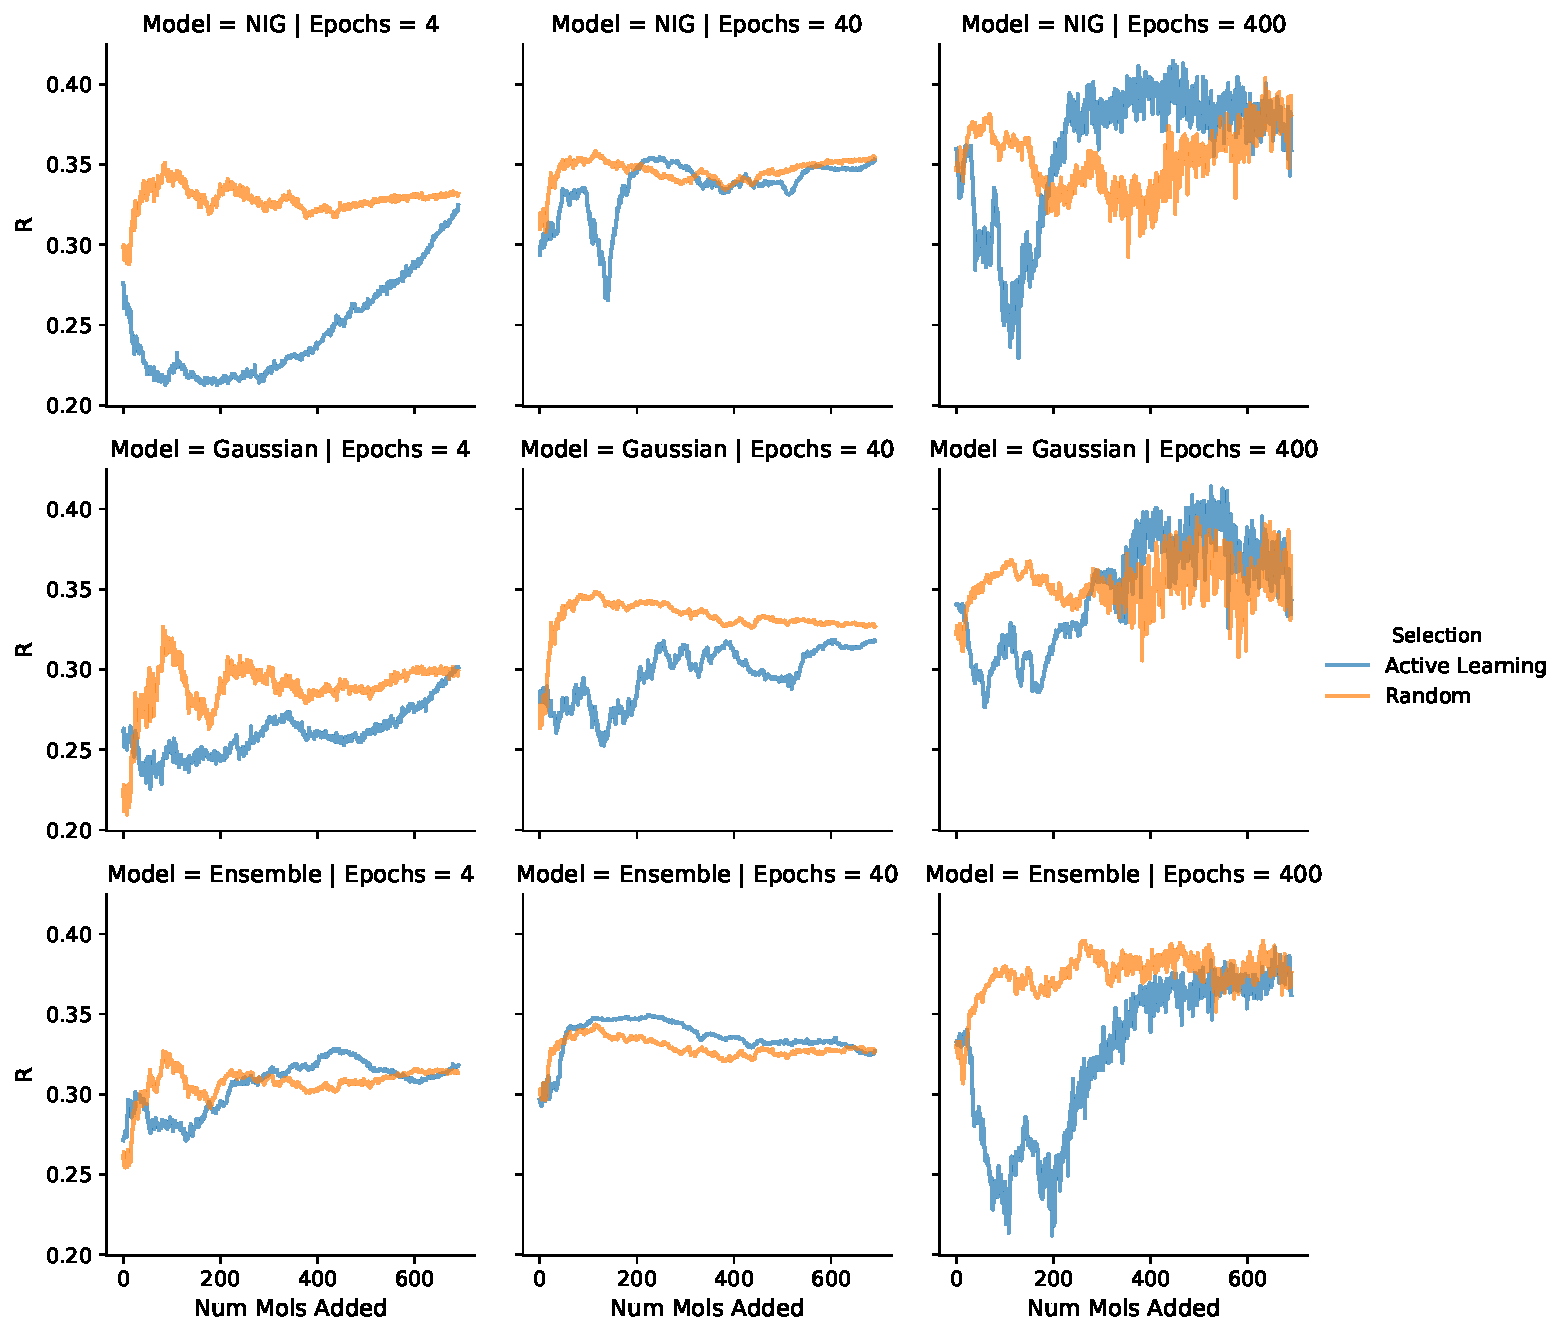
\includegraphics[width=1\linewidth]{figures/fig6_MAT_input_R_rest.pdf}
        \caption{Pearson's R correlation on the External Clusters}
    \end{subfigure}%
    \hfill
    \begin{subfigure}[b]{0.48\textwidth}
        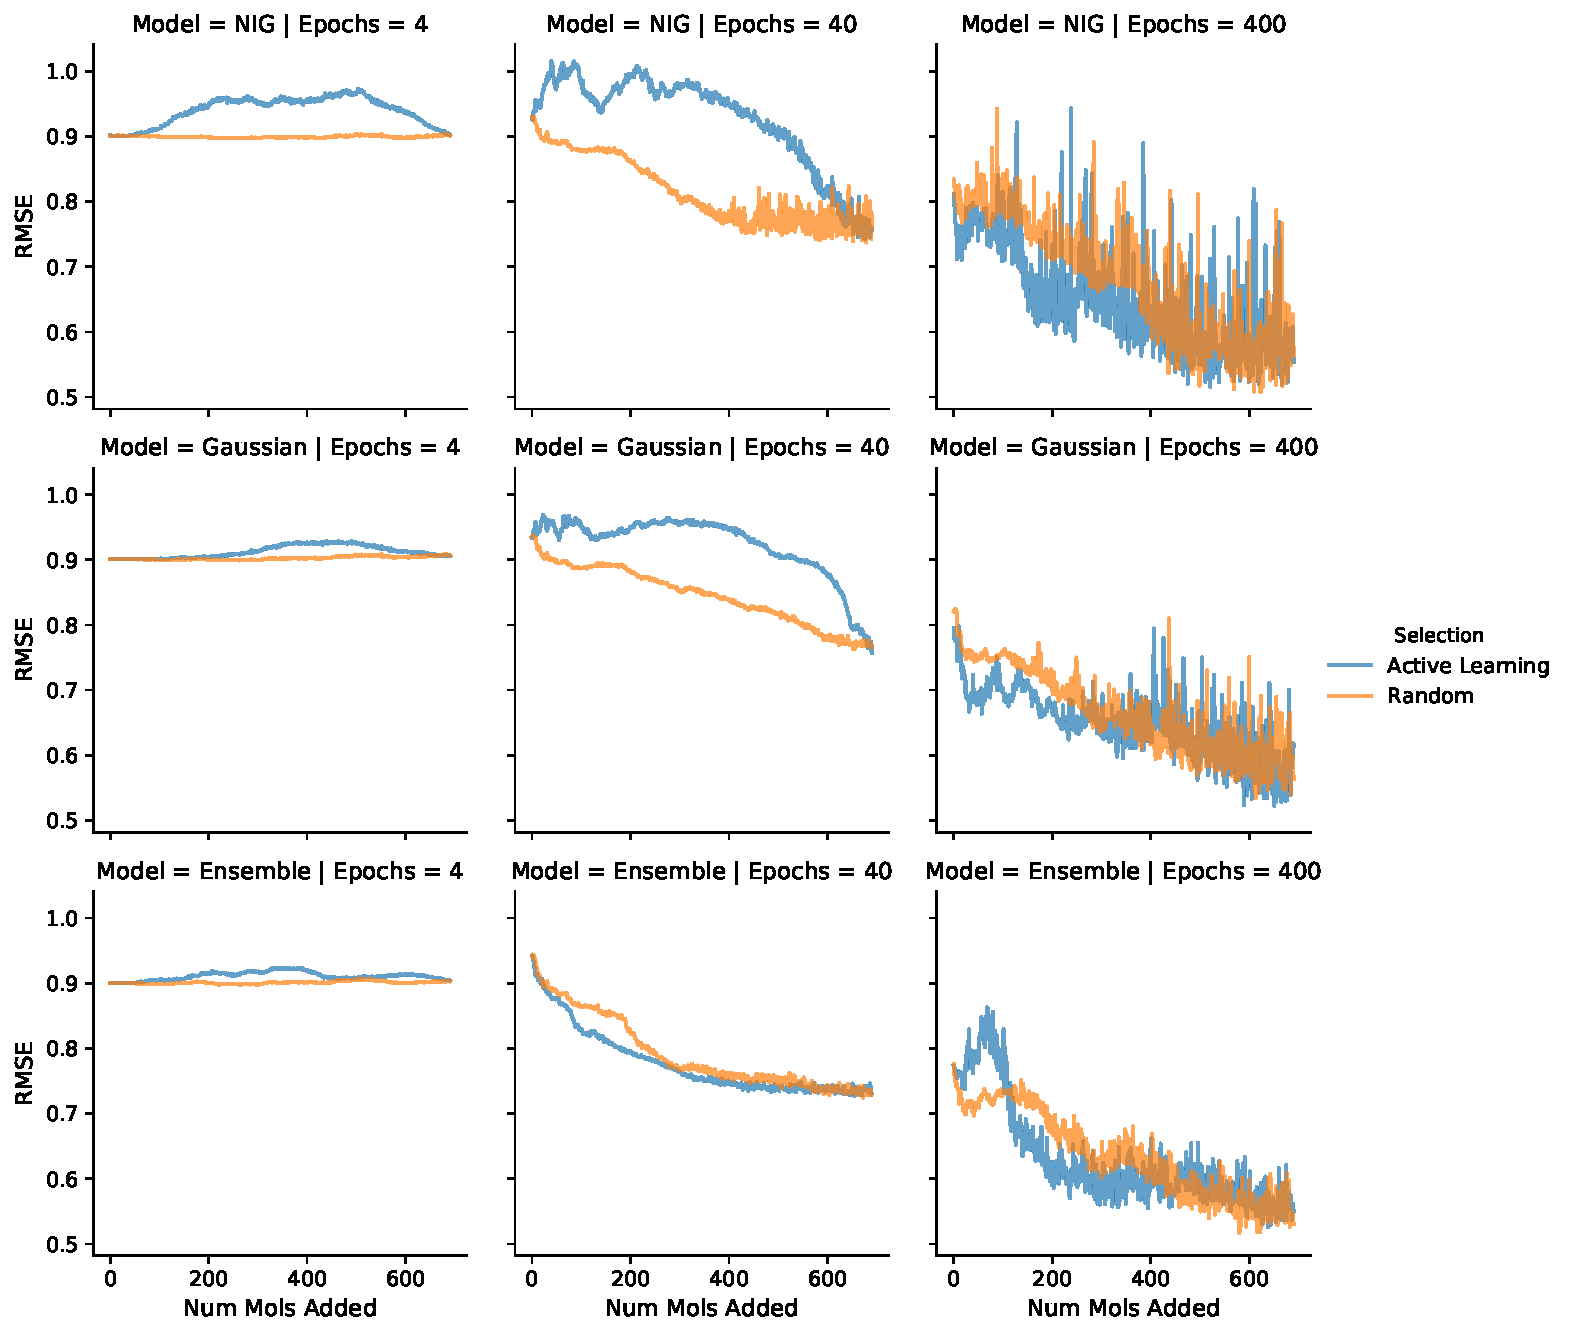
\includegraphics[width=1\linewidth]{figures/fig6_MAT_input_RMSE.pdf}
        \caption{Pearson's R correlation on the Test Set}
    \end{subfigure}%
    \hfill
    \begin{subfigure}[b]{0.48\textwidth}
        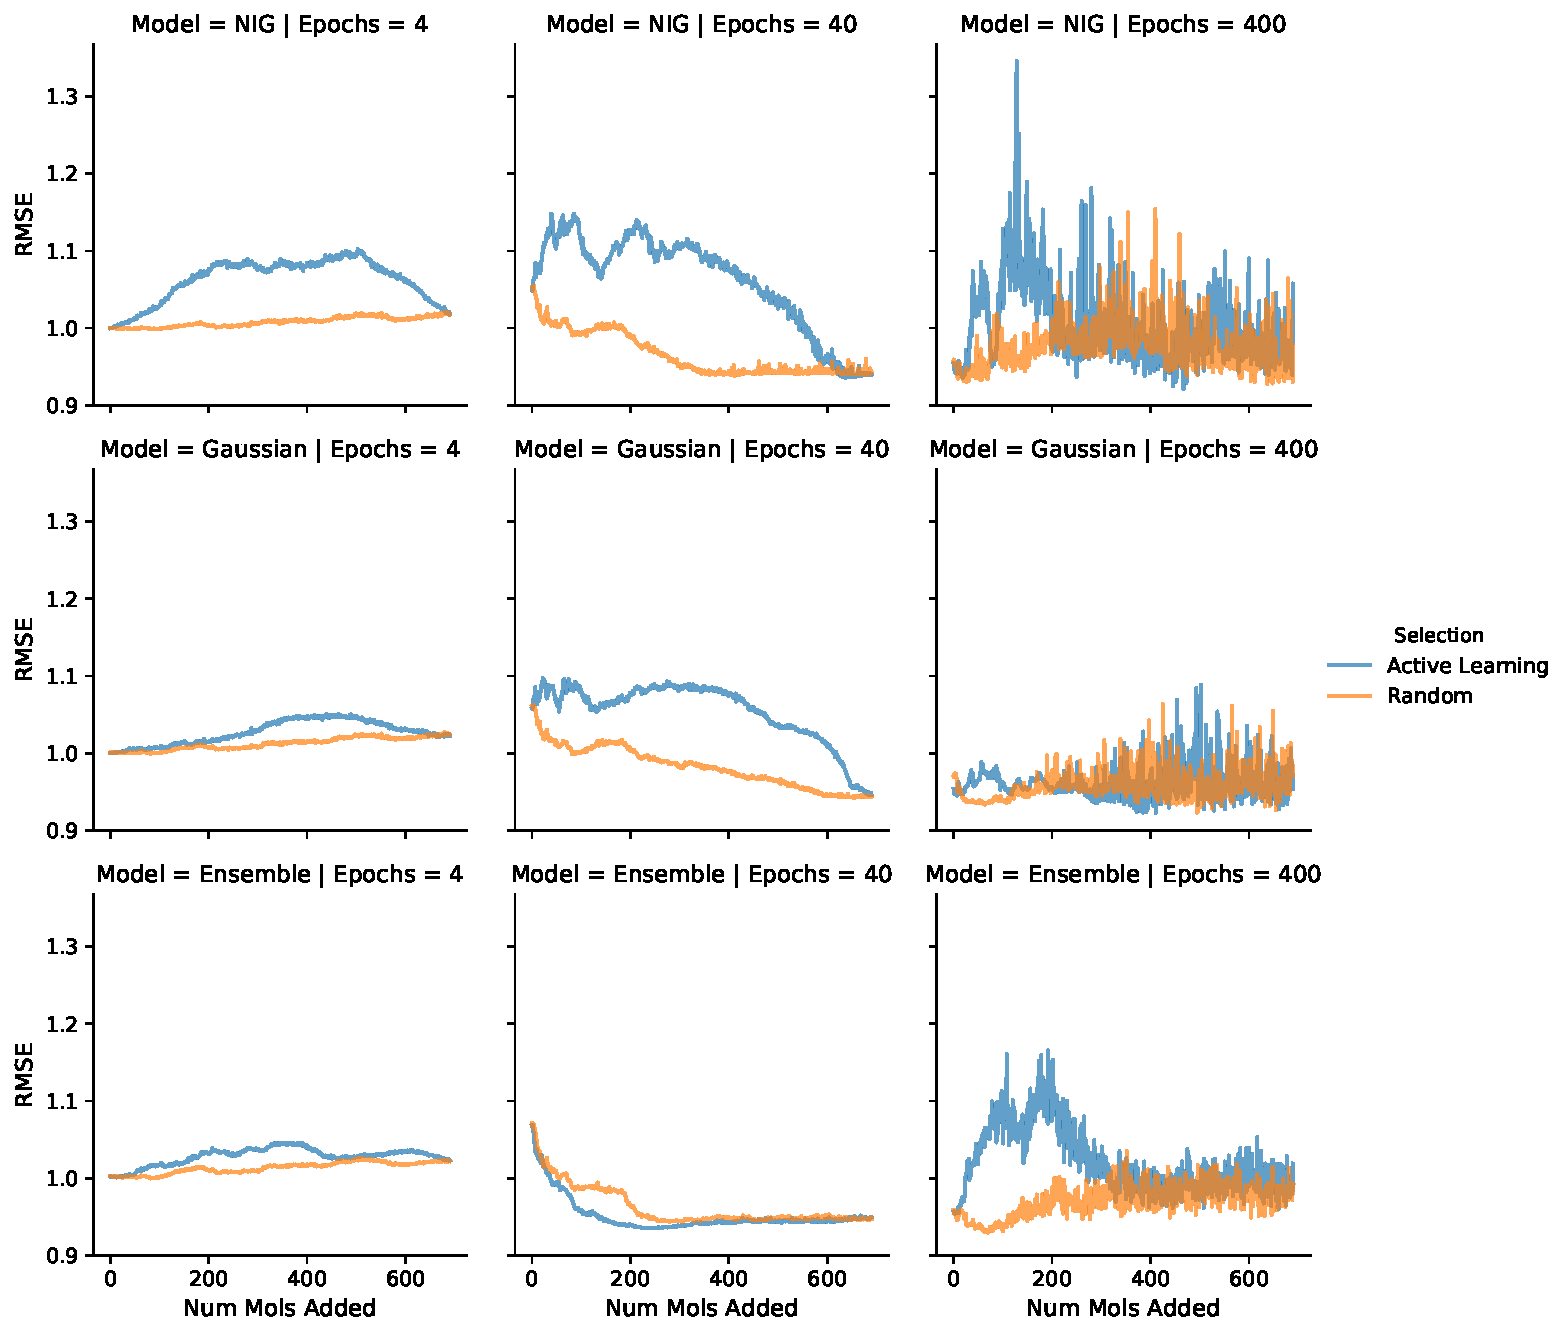
\includegraphics[width=1\linewidth]{figures/fig6_MAT_input_RMSE_rest.pdf}
        \caption{Pearson's R correlation on the External Clusters}
    \end{subfigure}
    \caption{Our sixth experiment testing the effect of a different input representation on the Clusters 02 dataset. In this experiment we only ran 1 seed on 1 fold of the data, but utilized every active learning approach. In each subgraph, a row contains an active learning approach, and the columns are the number of epochs the model trains. Again we find that the differing active learning approaches do not outperform picking molecules at random, and the overall model performance is unaffected.}
    \label{fig:MATinput}
\end{figure}

\subsection{Experiment 7 -- Verifying Transformer results}

In experiment 6 the 4 epoch trained NIG regression models show strange behavior with regards to the difference between the active learning and random selections. Specifically, the starting Pearson's R values are quite far apart, and the performance curve is flat, whereas for active learning the RMSE curve steadily gets worse. Thus we ran 4 additional seeds on 4 different splits of the "Largest Cluster 02" dataset with a 4 epoch trained NIG regression model using the MAT's generator output as input features. With the additional seeds we show that there is no difference between the active learning selection and selecting molecules at random (Figure~\ref{fig:expandedMAT})

\begin{figure}[tbph]
    \centering
    \begin{subfigure}[b]{0.48\textwidth}
        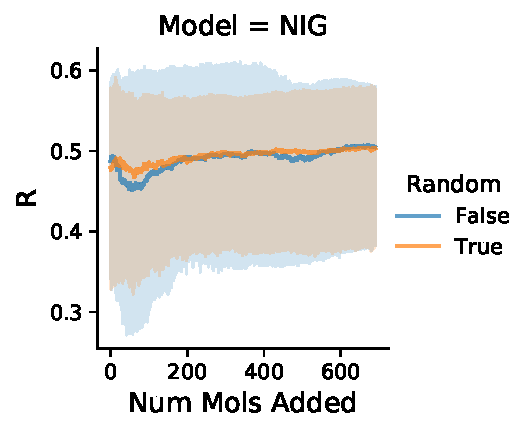
\includegraphics[width=1\linewidth]{figures/fig7_expanded_MAT_R.pdf}
        \caption{Pearson's R correlation on the Test Set}
    \end{subfigure}%
    \hfill
    \begin{subfigure}[b]{0.48\textwidth}
        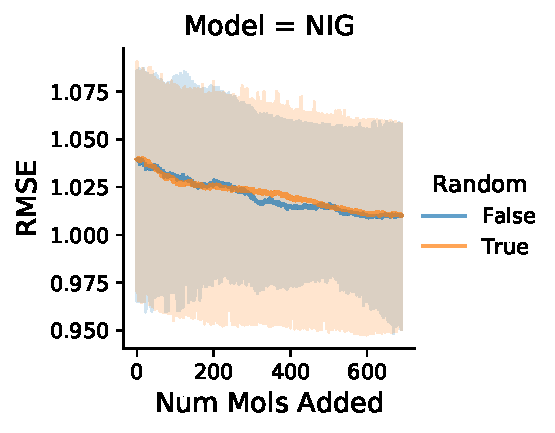
\includegraphics[width=1\linewidth]{figures/fig7_expanded_MAT_RMSE.pdf}
        \caption{RMSE on the Test Set}
    \end{subfigure}
    \caption{Our seventh experiment testing additional seeds for models using the MAT generator as input features. We show the R and RMSE results on the within cluster test set of the "Largest Cluster 02" for a 4 epoch trained model with regresses to a NIG distribution. The additional seeds allow us to conclude that there is no difference between active learning selection or selecting molecules at random.}
    \label{fig:expandedMAT}
\end{figure}

\subsection{Experiment 8 -- Using a much larger model}

Given the failures of Experiments 1 through 7 at generalization, and that larger models tend to generalize better \cite{bigmodelgeneralize}, we elected to take our earlier Morgan fingerprint based method and dramatically increase the number of layers in the model. The maximum number of hidden layers in our hyperparameter sweep was 4 (Figure~\ref{tab:archsweep}, so we evaluated the same general model architecture as our deployed model, but used 9 hidden layers instead. For this experiment we trained 1 seed on the "Largest Cluster 02" data split, and since this model is larger we also trained for 4, 40, or 400 epochs for each active learning selection method. The results of this experiment are shown in Figure~\ref{fig:bigmodel}. We find that there is minimal difference between picking molecules at random and using an active learning approach, and that the much larger model's final performance on the withheld clusters is similar to the results we found in Experiment 5 (Figure\ref{fig:lc02greed}. Thus, more than doubling the number of hidden layers in the model was insufficient to rescue the poor results we have observed.

\begin{figure}[tbph]
    \centering
    \begin{subfigure}[b]{0.48\textwidth}
        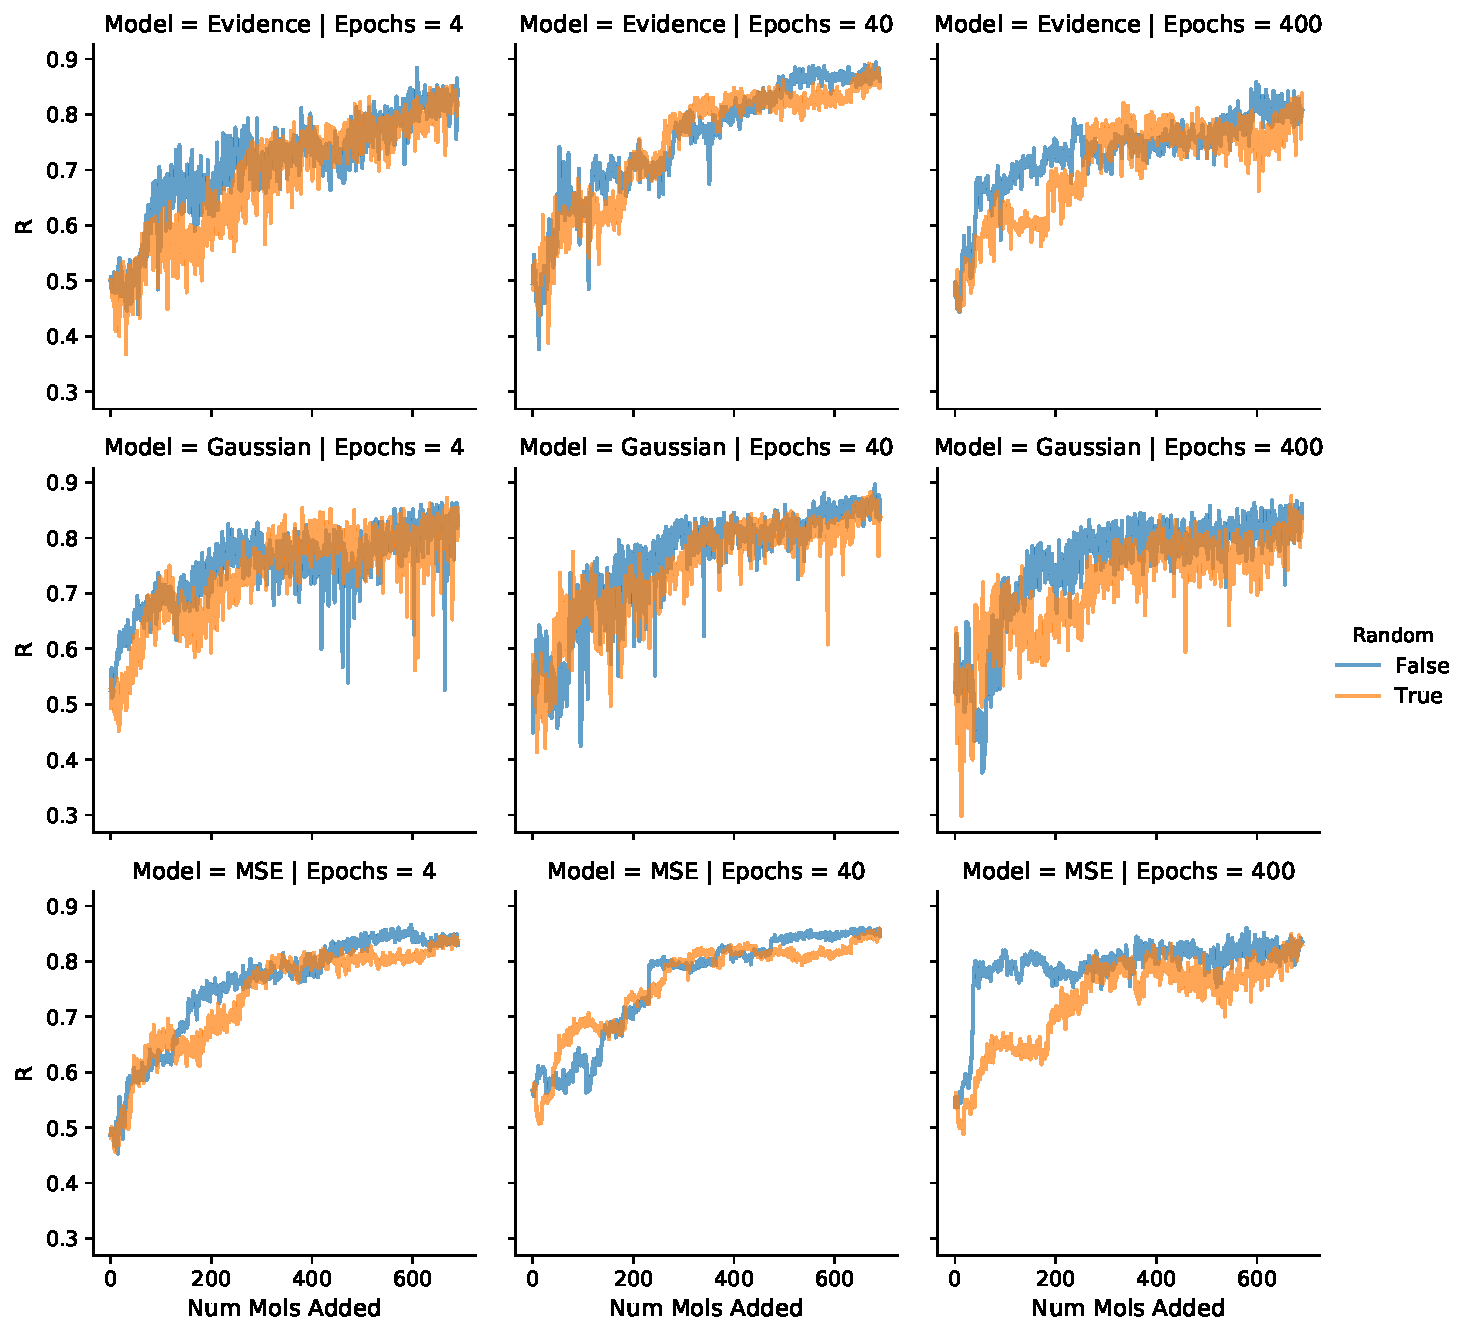
\includegraphics[width=1\linewidth]{figures/fig8_morgan_fp_bigmodel_R.pdf}
        \caption{Pearson's R correlation on the Test Set}
    \end{subfigure}%
    \hfill
    \begin{subfigure}[b]{0.48\textwidth}
        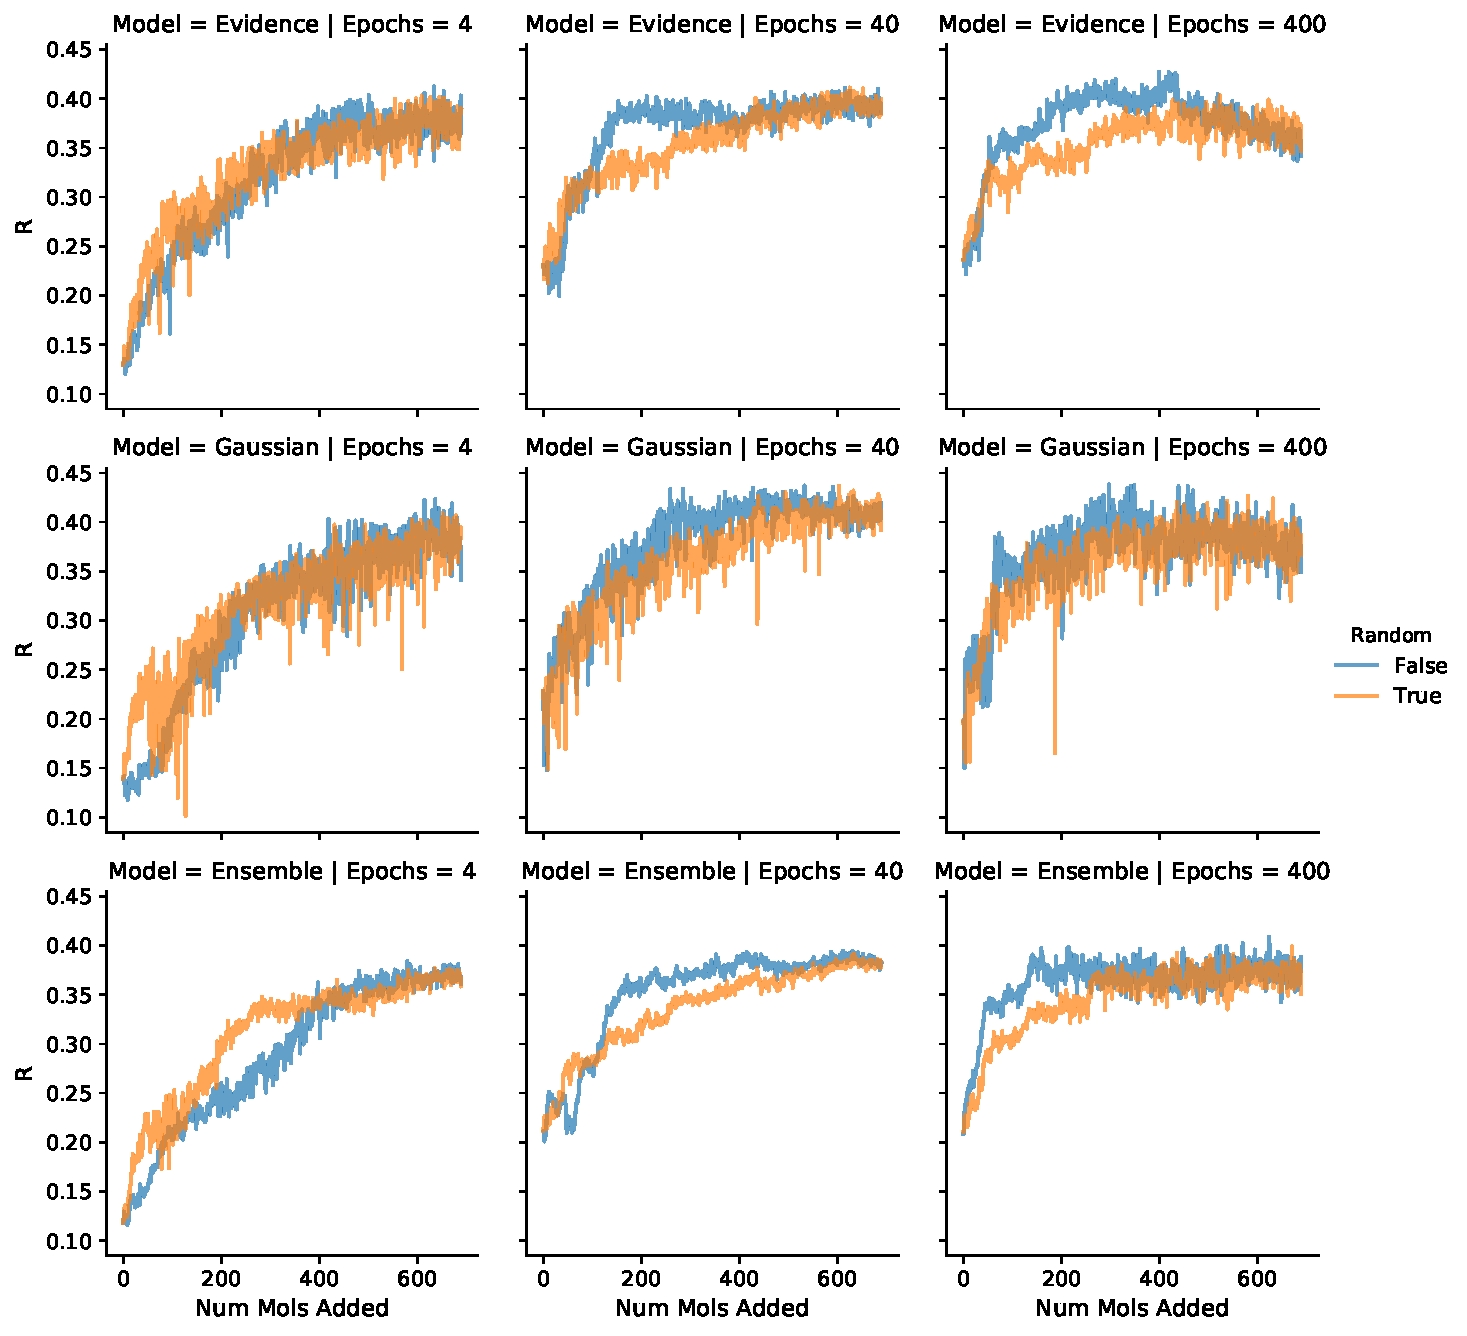
\includegraphics[width=1\linewidth]{figures/fig8_morgan_fp_bigmodel_rest_R.pdf}
        \caption{Pearson's R correlation on the External Clusters}
    \end{subfigure}%
    \hfill
    \begin{subfigure}[b]{0.48\textwidth}
        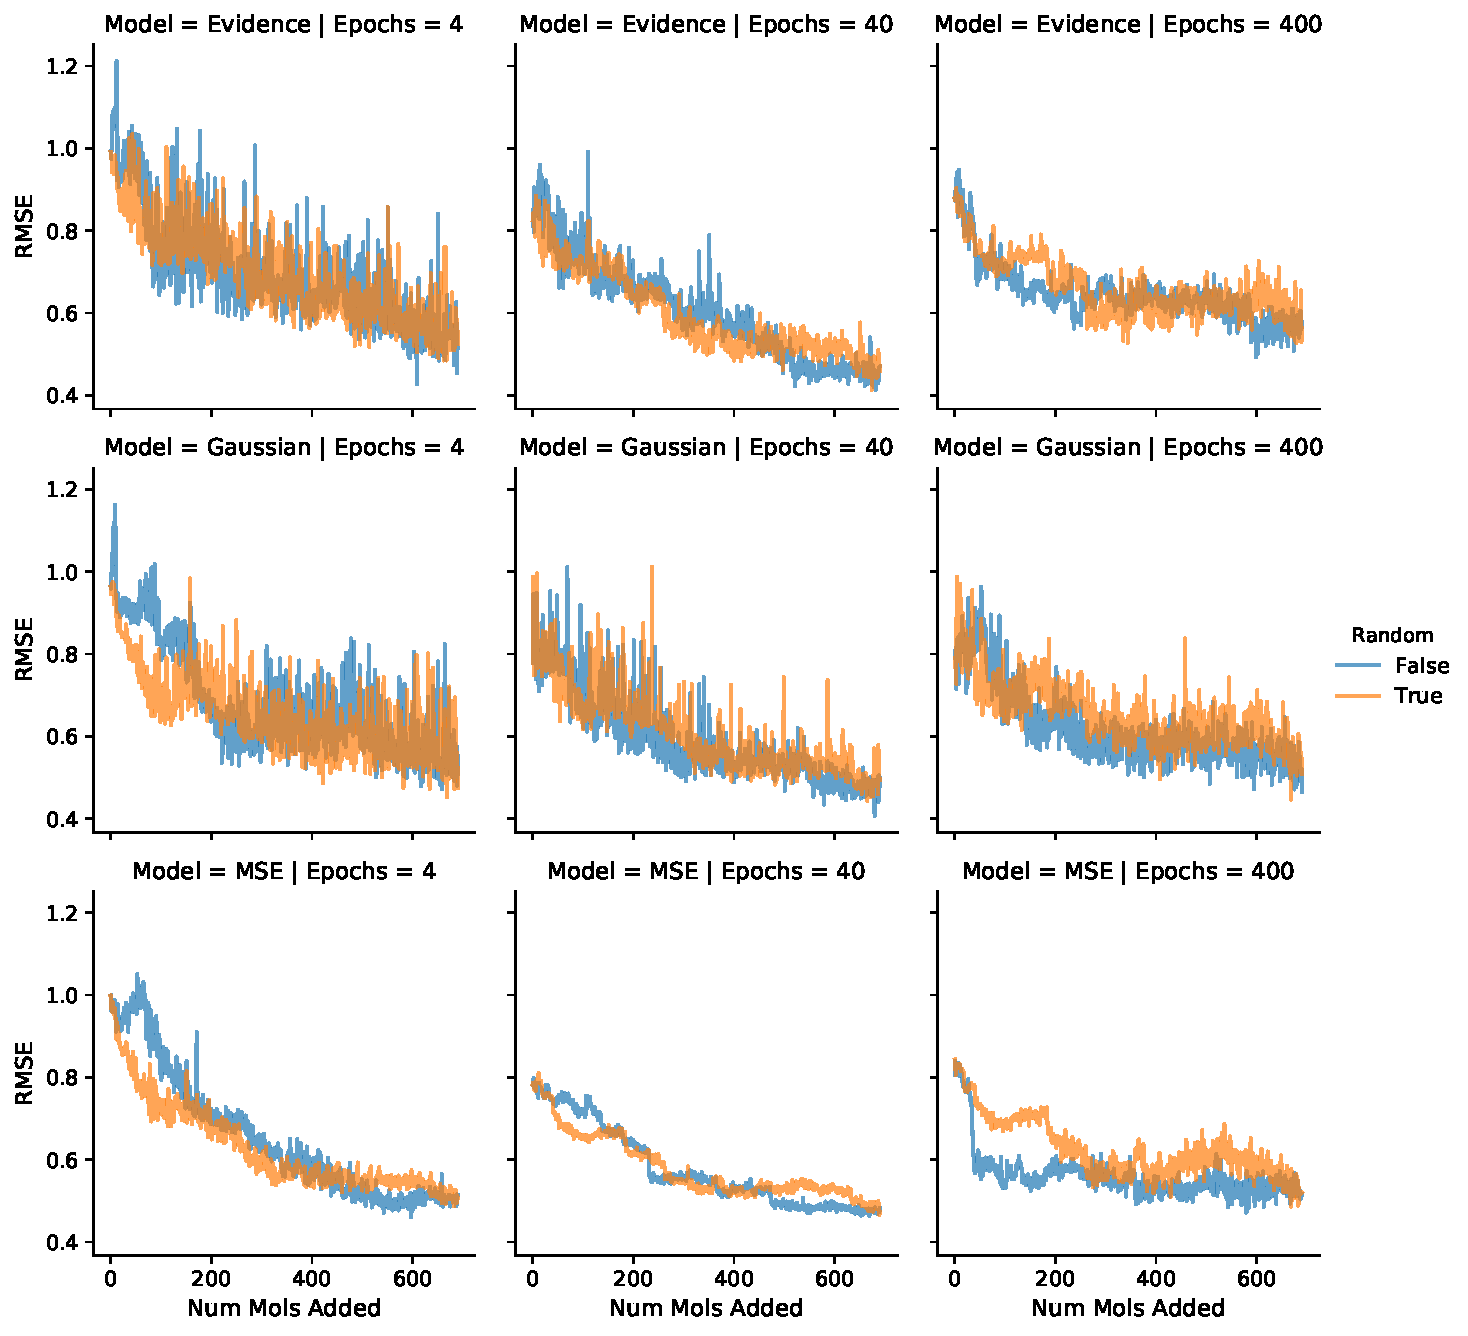
\includegraphics[width=1\linewidth]{figures/fig8_morgan_fp_bigmodel_RMSE.pdf}
        \caption{Pearson's R correlation on the Test Set}
    \end{subfigure}%
    \hfill
    \begin{subfigure}[b]{0.48\textwidth}
        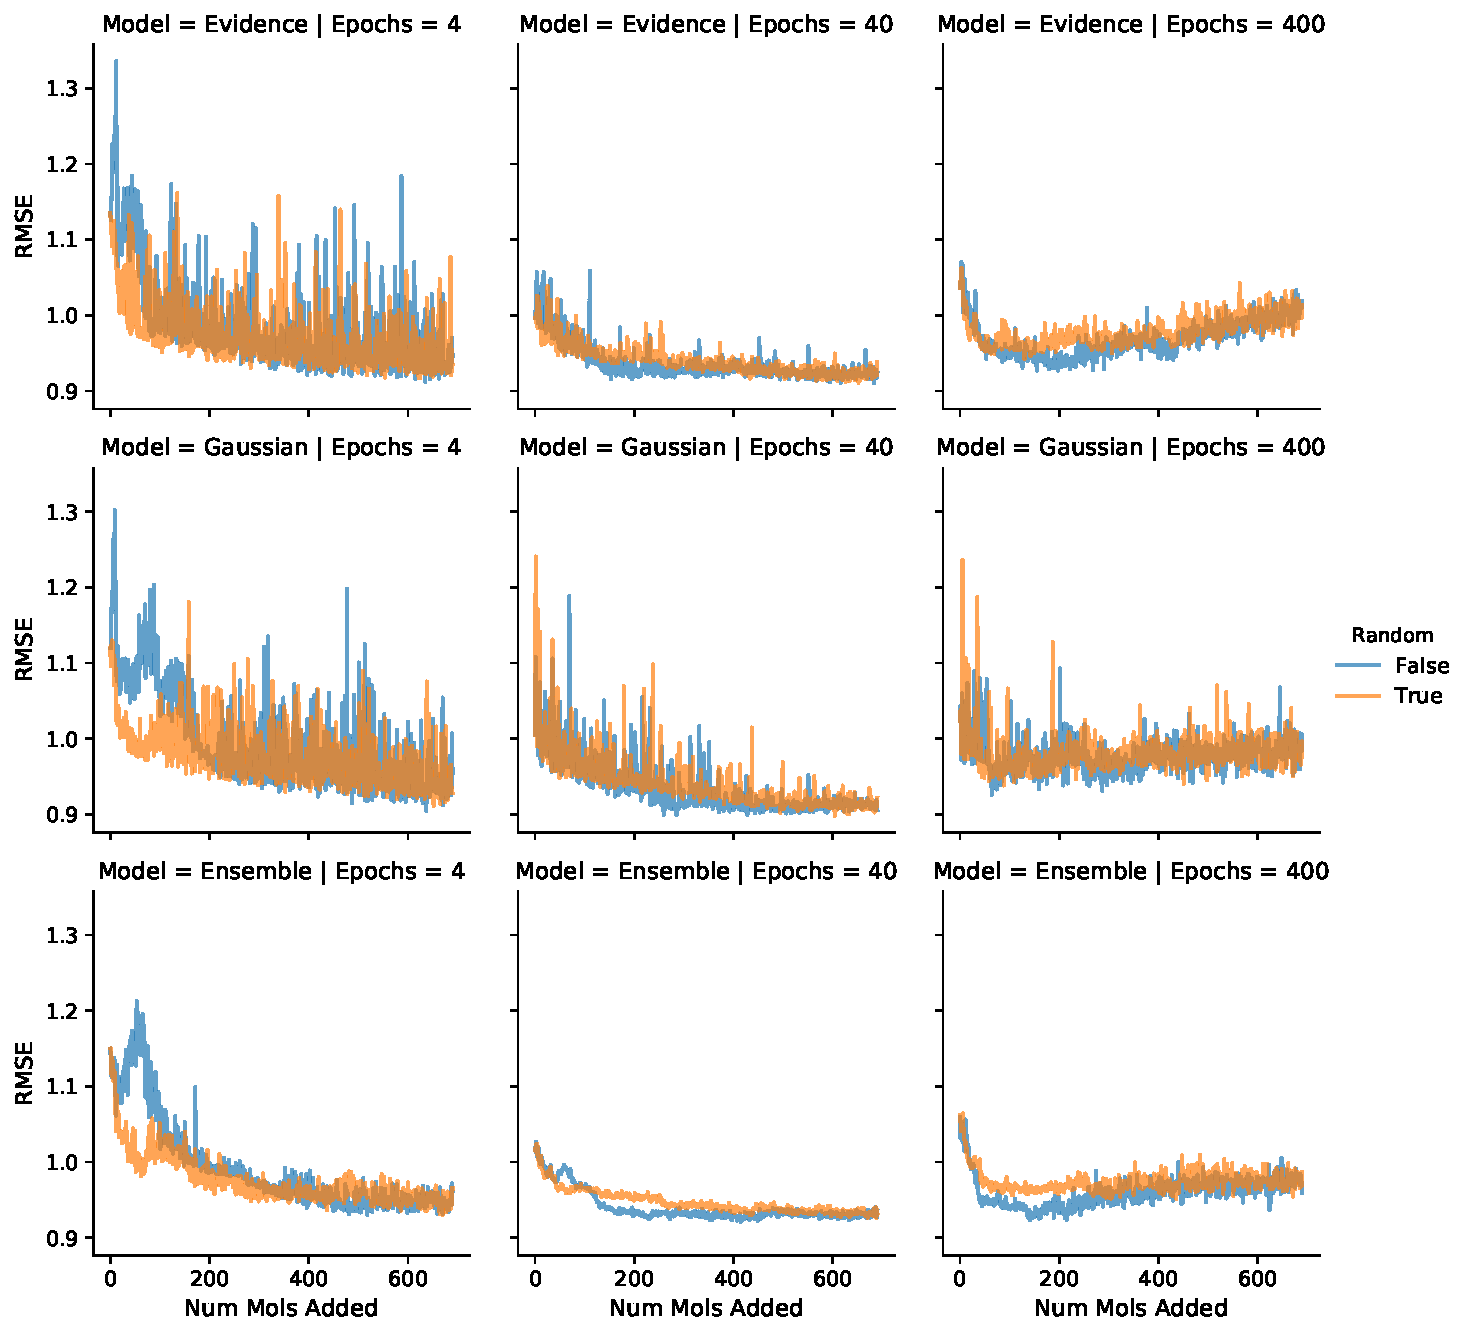
\includegraphics[width=1\linewidth]{figures/fig8_morgan_fp_bigmodel_rest_RMSE.pdf}
        \caption{Pearson's R correlation on the External Clusters}
    \end{subfigure}
    \caption{Our eighth experiment testing the effect of using a much larger fingerprint model on the Clusters 02 dataset. In this experiment we only ran 1 seed on 1 fold of the data, but utilized every active learning approach and trained for 4, 40, or 400 epochs. In each subgraph, a row contains an active learning approach, and the columns are the number of epochs the model trains. Again we find that the differing active learning approaches do not outperform picking molecules at random, and the final model performance is generally unaffected.}
    \label{fig:bigmodel}
\end{figure}

\subsection{Experiment 9 -- Implementing a new active learning selection criteria.}

All of our active learning selection methods are attempting to utilize a model's predicted uncertainty about the pool of unlabeled molecules in order to select the molecules that the model is most uncertain about to add to the training data. This approach is reasonable, but has failed to outperform random selection in all of our experiments. Thus, we experimented with a different active learning selection criteria. This new criteria selects new molecules based on the maximal absolute difference between the previous predicted label and the new predicted label. We hypothesize that the molecules whose predicted label changes the most between active learning cycles would thus be the most informative molecules to add to the training set. We implemented this selection criteria and evaluated models

\begin{itemize}
    \item \st{Ensemble variance, Gaussian Regression, NIG regression over all CCV data}
    \item \st{as above, but restricted to 1 cluster}
    \item \st{Baseline experiment to determine if signal is present -- Greedy line}
    \item \st{1cluster Train/withheld/valid/test}
    \item \st{Using 2 clusters}
    \item \st{Varying training times and input representations -- Transformer}
    \item \st{checking 5 seeds of Transformer input}
    \item \st{Using a much larger model}
    \item changing AL selection criteria 
    \item Batching molecules for selection
\end{itemize}

%%%%%%%%%%%%%%%%%%%%%%%%%%%%%%%%%%%%%%%%%%%%%%%%%%%%%%%%%%%%%%%%%%%%%
%% Discussion
%%%%%%%%%%%%%%%%%%%%%%%%%%%%%%%%%%%%%%%%%%%%%%%%%%%%%%%%%%%%%%%%%%%%%
\section{Discussion}

womp womp

%%%%%%%%%%%%%%%%%%%%%%%%%%%%%%%%%%%%%%%%%%%%%%%%%%%%%%%%%%%%%%%%%%%%%
%% The "Acknowledgement" section can be given in all manuscript
%% classes.  This should be given within the "acknowledgement"
%% environment, which will make the correct section or running title.
%%%%%%%%%%%%%%%%%%%%%%%%%%%%%%%%%%%%%%%%%%%%%%%%%%%%%%%%%%%%%%%%%%%%%
\begin{acknowledgement}


The authors thank <insert names here> for their insightful contributions during the preparation of this manuscript.

This work is supported by R35GM140753 from the National Institute of General Medical Sciences. The content is solely the responsibility of the authors and does not necessarily represent the official views of the National Institutes of Health.

\end{acknowledgement}

%%%%%%%%%%%%%%%%%%%%%%%%%%%%%%%%%%%%%%%%%%%%%%%%%%%%%%%%%%%%%%%%%%%%%
%% The same is true for Supporting Information, which should use the
%% suppinfo environment.
%%%%%%%%%%%%%%%%%%%%%%%%%%%%%%%%%%%%%%%%%%%%%%%%%%%%%%%%%%%%%%%%%%%%%
%\begin{suppinfo}

%This will usually read something like: ``Experimental procedures and
%characterization data for all new compounds. The class will
%automatically add a sentence pointing to the information on-line:
%Supporting Information Available: Supplementary Figures (\ref{fig:hyperparamters}-\ref{fig:rotensemble}), Tables (\ref{tab:trainhyper}-\ref{tab:RedCD2020}), and Methods.
%\end{suppinfo}

%%%%%%%%%%%%%%%%%%%%%%%%%%%%%%%%%%%%%%%%%%%%%%%%%%%%%%%%%%%%%%%%%%%%%
%% The appropriate \bibliography command should be placed here.
%% Notice that the class file automatically sets \bibliographystyle
%% and also names the section correctly.
%%%%%%%%%%%%%%%%%%%%%%%%%%%%%%%%%%%%%%%%%%%%%%%%%%%%%%%%%%%%%%%%%%%%%
\bibliography{references}

\end{document}